\documentclass[a4paper,12pt,oneside,onecolumn]{article}
\usepackage[utf8]{inputenc}
\usepackage[italian]{babel}
\usepackage{hyperref}
\usepackage[round,numbers]{natbib}
\usepackage{textcomp}
%\usepackage{listings}
\usepackage{graphicx}
\usepackage{caption}
\usepackage{subcaption}
%\usepackage{amsmath}
\usepackage[T1]{fontenc}
\usepackage{lmodern}
%\usepackage[scaled=0.9]{beramono}
%\usepackage{microtype}
\usepackage{color}
\usepackage{xcolor}
%\usepackage{float}
\usepackage{multirow}
\usepackage{lipsum}
\usepackage[noadvisor,swapnames]{frontespizio}
\usepackage{minted}
\definecolor{light-gray}{gray}{0.95}
\usepackage{booktabs}
\usepackage{appendix}
\renewcommand{\appendixtocname}{Appendici}
\renewcommand{\appendixpagename}{Appendici}
\usepackage{multicol}
%\setlength{\columnsep}{.5cm}
\renewcommand*\rmdefault{iwona}

\usepackage{algorithm}
\usepackage{algorithmic}
\usepackage{csvsimple}
\usepackage{pgfplotstable}

\usemintedstyle{default}

\newminted{prolog}
{ 
  frame=lines,
  framesep=2mm,
  baselinestretch=1,
  bgcolor=light-gray,
  fontsize=\small,
  linenos
}

\newminted{java}
{ 
  frame=lines,
  framesep=2mm,
  baselinestretch=1,
  bgcolor=light-gray,
  fontsize=\footnotesize,
  linenos
}

\newminted{python}
{ 
  frame=lines,
  framesep=2mm,
  baselinestretch=1,
  bgcolor=light-gray,
  fontsize=\footnotesize,
  linenos
}

\begin{document}

    \begin{frontespizio}
        \Universita {Bari ``Aldo Moro"}
        \Logo [2cm]{./img/logo}
        \Dipartimento{Informatica}
        \Corso [Laurea]{Informatica Magistrale}
        \Titoletto {Documentazione di progetto di Intelligenza Artificiale}
        \Titolo{Sperimentazioni FOIL - ALEPH - PROGOL}
        \NCandidati{Studenti}
        \Candidato{Luciano Quercia}
        \Candidato{Simone Rutigliano}
        \Annoaccademico {2013-2014}
        \Margini{3cm}{4cm}{3cm}{3.5cm}
    \end{frontespizio}

\tableofcontents

\section{DATASETS}
\begin{table}[htbp]
	\centering
	\begin{tabular}{cccc}
		Elsevier & + 61 & Tot: 353 & \%+ 21\% \\
		 & -292 &  & \\
		 \hline
		 JMLR & +100 & Tot: 353 & \%+ 40\% \\
		 & -253 & & \\
 		 \hline
 		 MLJ & +122 & Tot: 353 & \%+ 53\% \\
 		 & -231 & & \\
 		 \hline
 		 SVLN & +70 & Tot: 353 & \%+ 25\% \\
 		 & -283 & & \\
		\end{tabular}%
	\label{tab:}
\end{table}
\subsection{ELSEVIER}
\begin{table}[htbp]
	\centering
		\begin{tabular}{cccccccccccc}
			FOLD &| &  0 &  1 &  2 &  3 &  4 &  5 &  6 &  7 &  8 &  9 \\ \hline
			Doc  &| & 35 & 35 & 35 & 35 & 35 & 35 & 35 & 36 & 36 & 36 \\
			Pos  &| & 6  & 6  &  6 &  6 &  6 &  6 &  6 &  6 &  6 &  7 \\
			Neg  &| & 29 & 29 & 29 & 29 & 29 & 29 & 29 & 30 & 30 & 29 \\
		\end{tabular}%
	\label{tab:Elsevier}
\end{table}
\subsection{JMLR}
\begin{table}[htbp]
	\centering
		\begin{tabular}{cccccccccccc}
			FOLD &| &  0 &  1 &  2 &  3 &  4 &  5 &  6 &  7 &  8 &  9 \\ \hline
			Doc  &| & 35 & 35 & 35 & 35 & 35 & 35 & 35 & 36 & 36 & 36 \\
			Pos  &| & 10  & 10  &  10 &  10 &  10 &  10 &  10 &  10 &  10 &  10 \\
			Neg  &| & 25 & 25 & 25 & 25 & 25 & 25 & 25 & 26 & 26 & 26 \\
		\end{tabular}%
	\label{tab:JMLR}
\end{table}
\subsection{MLJ}
\begin{table}[htbp]
	\centering
	%
		\begin{tabular}{cccccccccccc}
			FOLD & | &  0 &  1 &  2 &  3 &  4 &  5 &  6 &  7 &  8 &  9 \\ \hline
			Doc  & | & 35 & 35 & 35 & 35 & 35 & 35 & 35 & 36 & 36 & 36 \\
			Pos  & | & 12  & 12  &  12 &  12 &  12 &  12 &  12 &  12 &  13 &  13 \\
			Neg  & | & 23 & 23 & 23 & 23 & 23 & 23 & 23 & 24 & 24 & 24 \\
		\end{tabular}%
	
	\label{tab:MLJ}
\end{table}
\subsection{SVLN}
\begin{table}[htbp]
	\centering
		\begin{tabular}{cccccccccccc}
			FOLD &| &  0 &  1 &  2 &  3 &  4 &  5 &  6 &  7 &  8 &  9 \\\hline
			Doc  &| & 35 & 35 & 35 & 35 & 35 & 35 & 35 & 36 & 36 & 36 \\
			Pos  &| & 7  & 7  &  7 &  7 &  7 &  7 &  7 &  7 &  7 &  7 \\
			Neg  &| & 28 & 28 & 28 & 28 & 28 & 28 & 28 & 29 & 29 & 29 \\
		\end{tabular}%
	\label{tab:SVLN}
\end{table}

\section{Sistemi di apprendimento}

I sistemi di apprendimento presi in esame saranno di tre tipi differenti:

\begin{itemize}
	\item ALEPH (A Learning Engine for Proposing Hypothesis)
	\item Progol 
	\item FOIL (First Order Inductive Learner)
\end{itemize}

\subsection{ALEPH}
Aleph is an acronym for "A Learning Engine for Proposing Hypotheses" and an Inductive Logic Programming (ILP) system. Aleph’s main purpose was to understand the concept of inverse entailment, which appeared in [2]. Aleph requires three files to construct theories. They are “filestem.b, filestem.f, and filestem.n,” which stand for background knowledge file, positive example file, and negative example file, respectively. Aleph receives these three files in order to construct a theory that is consistent with positive examples and inconsistent with negative ones.
The background knowledge inputted into Aleph is generated by means of Case-Based Reasoning (CBR) with user interaction if necessary. Sophisticated background knowledge should be provided to efficiently process natural language documents since they are rich in representation. The acquisition of background knowledge is one of the problems to be overcome. On the other hand, the acquisition and compilation of background knowledge have been reported to cause a bottleneck in knowledge engineering because they are very time-consuming tasks. The automatic generation of background knowledge provides a solution to the problem.

\subsection{Progol}
Progol is an implementation of Inductive Logic Programming used in computer science that combines "Inverse Entailment" with "general-to-specific search" through a refinement graph. [1][2][3] "Inverse Entailment" is used with mode declarations to derive the most-specific clause within the mode language which entails a given example. This clause is used to guide a refinement-graph search.

Unlike the searches of Ehud Shapiro's Model Inference System (MIS) and J. Ross Quinlan's FOIL Progol's search is efficient and has a provable guarantee of returning a solution having the maximum "compression" in the search-space. To do so it performs an admissible A*-like search, guided by compression, over clauses which subsume the most specific clause.

Progol deals with noisy data by using the "compression measure" to trade-off the description of errors against the hypothesis description length. Progol allows arbitrary Prolog programs as background knowledge and arbitrary definite clauses as examples. Despite this bench-tests show that the efficiency of Progol compares favourably with FOIL.
\nocite{wiki:progol}
%WIKIPEDIA 

P-Progol is intended to be a prototype for exploring ideas. It commenced in 1993 as part of a fun project undertaken by Ashwin Srinivasan and Rui Camacho at Oxford University. The main purpose was to understand ideas of inverse entailment which eventually appeared in Steve Muggleton's paper, and was accompanied by (good-natured) bun-fights about the execution speeds of programs being written by Ashwin (who was writing P-Progol) and Rui (who was writing Indlog). The earliest P-Progol implementation dates from April, 1993. There are, currently, at least 3 implementations based on the Progol algorithm: CProgol (by S. Muggleton, written in C which contains its own Prolog interpreter), Indlog (by Rui Camacho, in Prolog requiring the Yap compiler) and P-Progol (by Ashwin Srinivasan, in Prolog largely developed with Yap). The main differences in implementation (other than language) are in the search technique used and degree of user-interaction allowed

The basic P-Progol algorithm
During routine use, P-Progol follows a very simple procedure that can be described in 4 steps:
Select example. Select an example to be generalised. If none exist, stop, otherwise proceed to the next step.
Build most-specific-clause. Construct the most specific clause that entails the example selected, and is within language restrictions provided. This is usually a definite clause with many literals, and is called the "bottom clause." This step is sometimes called the "saturation" step.
Search. Find a clause more general than the bottom clause. This is done by searching for some subset of the literals in the bottom clause that has the "best" score. Two points should be noted. First, confining the search to subsets of the bottom clause does not produce all the clauses more general than it, but is good enough for this thumbnail sketch. Second, the exact nature of the score of a clause is not really important here. This step is sometimes called the "reduction" step.
Remove redundant. The clause with the best score is added to the current theory, and all examples made redundant are removed. This step is sometimes called the "cover removal" step. Note here that the best clause may make clauses other than the examples redundant. Again, this is ignored here. Return to Step 1.
P-Progol is an implementation based around these 4 steps. A more advanced use of P-Progol (see section Advanced use of P-Progol) allows alteration to each of these steps.


\subsection{FOIL}
\nocite{Quinlan:1993:FMR:645323.649599}
FOIL è un sistema di apprendimento in grado di costruire delle clausole di Horn a partire da esempi sia positivi che negativi.
%FOIL is a learning system that constructs Horn clause programs from examples.
%FOIL is a system for learning function-free Horn clause definitions of a relation in terms of itself and other relations.

The principal differences between zeroth-order and first-order supervised learning systems are the form of the training data and the way that a learned theory is expressed. Data for zeroth-order learning programs such as CN2 and C4.5 Quinlan, 1992 comprise preclassi ed cases, each described by its values for a xed collection of attributes.
These systems develop theories, in the form of decision trees or production rules, that relate a case's class to its attribute values. In contrast, the input to first-order learners (usually) contains ground assertions about a number of multi-argument predicates or relations and the learned theory consists of a logic program, restricted to Horn clauses or something similar, that predicts when a vector of arguments will satisfy a designated predicate.
FOIL uses a divide-and-cover strategy adapted from zeroth-order learning. These approaches have proved to be more e cient and robust, enabling larger training sets to be analysed to learn more complex programs.

The program is actually slightly more exible since it can learn several relations in sequence, allows negated literals in the de nitions (using standard Prolog semantics), and can employ certain constants in the de nitions it produces.
FOIL 's input consists of information about the relations, one of which (the target
relation ) is to be de ned by a Horn clause program. For each relation it is given
a set of tuples of constants that belong to the relation. For the target relation
it might also be given tuples that are known not to belong to the relation;
alternatively, the closed world assumption may be invoked to state that no tuples,
other than those speci ed, belong to the target relation. Tuples known to be in
the target relation will be referred to as tuples and those not in the relation as
tuples. The learning task is then to nd a set of clauses for the target relation
that accounts for all the tuples while not covering any of the tuples.
The basic approach used by FOIL is an AQ-like covering algorithm Michalski,
Mozetic, Hong and Lavrac, 1986]. It starts with a training set containing all
and tuples, constructs a function-free Horn clause to `explain' some of the
tuples, removes the covered tuples from the training set, and continues with
the search for the next clause. When clauses covering all the tuples have been
found, they are reviewed to eliminate any redundant clauses and reordered so
that any recursive clauses come after the non-recursive base cases.
Perfect de nitions that exactly match the data are not always possible, particu-
larly in real-world situations where incorrect values and missing tuples are to be
expected. To get around this problem, FOIL uses encoding-length heuristics tolimit the complexity of clauses and programs. The nal clauses may cover most
(rather than all) of the tuples while covering few (rather than none) of the
tuples. See Quinlan, 1990] for details.

\section{Dataset utilizzati}

I tre sistemi precedentemente descritti verranno testati su quattro dataset.

\subsection{Dominio e provenienza}
I dataset sono stati generati per task inerenti alla Document Image Understanding.
Contengono la descrizione, sotto forma di clausole di Horn, di componenti di documenti testuali opportunamente analizzate.

I dataset contengono le informazioni su paper scientifici provenienti da 4 journal:
\begin{itemize}
\item Elsevier journals (Elsevier)
\item Springer-Verlag Lecture Notes (SVLN)
\item Journal of Machine Learning Research (JMLR)
\item Machine Learning Journal (MLJ).
\end{itemize}

\subsection{Descrizione}
I \emph{documenti} sono tutti composti da una sola \emph{pagina}. Ogni \emph{pagina} contiene un numero variabile di \emph{frame}, ossia rettangoli all'interno del paper (e.g. titolo, abstract, paragrafo, logo).

Tutte le informazioni contenute nei dataset riguardano una di queste tre entità (documento, pagina, frame) e le relazioni esistenti fra esse.

Le proprietà utilizzate sono riportate in tabella \ref{tab:proprieta}

\begin{table}[h!tbp]
\centering
\footnotesize\begin{tabular}{lccl}
\toprule
\addlinespace
Nome proprietà & Arg 1 & Arg 2 & Descrizione \\
\addlinespace
\midrule
\addlinespace
numero\_pagine & Doc & Int & Numero di pagine del Documento \\ 
pagina\_1 & Doc & Page & Prima pagina del documento \\ 
ultima\_pagina & Page & - & Ultima pagina del documento\\
frame & Page & Frame & Frame all'interno della pagina\\
allineato\_al\_centro\_orizzontale & Frame & Frame & I frame sono allineati orizz.\\
allineato\_al\_centro\_verticale & Frame & Frame & I frame sono allineati vert.\\
altezza\_pagina & Page & Float & Altezza della pagina\\
larghezza\_pagina & Page & Float & Larghezza della pagina\\
altezza\_rettangolo & Frame & Float & Altezza delf rame\\
larghezza\_rettangolo & Frame & Float & Larghezza del Frame\\
ascissa\_rettangolo & Frame & Float & Posizione orizzontale del frame\\
ordinata\_rettangolo & Frame & Float & Posizione verticale del frame\\
on\_top & Frame & Frame & Primo frame sopra al secondo\\
to\_right & Frame & Frame & Primo Frame alla destra del secondo\\
tipo\_immagine & Frame & - & Il frame contiene un'immagine\\
tipo\_linea\_obbliqua & Frame & - & Il frame contiene una linea obliqua\\
tipo\_linea\_orizzontale & Frame & - & Il frame contiene linea orizzontale\\
tipo\_misto & Frame & - & Il frame contiene componenti varie\\
tipo\_testo & Frame & - & Il frame contiene solo testo\\
tipo\_vuoto & Frame & - & Il frame è vuoto\\
\addlinespace
\bottomrule 
\end{tabular}
\caption[Proprietà]{Nomi, argomenti e descrizione delle proprietà presenti nei dataset.}
\label{tab:proprieta}
\end{table}

Solo nel caso del dataset \emph{MLJ}, abbiamo avuto a disposizione un file contenente gli intervalli di discretizzazione delle 4 componenti numeriche delle seguenti proprietà
\begin{itemize}
\item altezza\_rettangolo
\item larghezza\_rettangolo
\item ascissa\_rettangolo
\item ordinata\_rettangolo
\end{itemize}
.

Solo per \emph{MLJ}, dunque, abbiamo potuto effettuare due sperimentazioni (con valori discretizzati e non). Per farlo, abbiamo eliminato le 4 proprietà numeriche e aggiunto 24 nuove proprietà.

\verb+altezza_rettangolo+ è stata divisa in $11$ bin, \verb+larghezza_rettangolo+ in $7$ bin, \verb+ascissa_rettangolo+ e \verb+ordinata_rettangolo+ in $3$ bin.

I nomi delle proprietà aggiunte sono riportate in tabella \ref{tab:discretizzazione}.

\begin{table}[h!tbp]
\centering
\small\begin{tabular}{lc}
\toprule
\addlinespace
Nome proprietà & Argomento \\
\addlinespace
\midrule
\addlinespace
height\_smallest & Frame \\ 
height\_very\_very\_small & Frame \\ 
height\_very\_small & Frame \\ 
height\_small & Frame \\ 
height\_medium\_small & Frame \\ 
height\_medium & Frame \\ 
height\_medium\_large & Frame \\ 
height\_large & Frame \\ 
height\_very\_large & Frame \\ 
height\_very\_very\_large & Frame \\ 
height\_largest & Frame \\ 
\midrule
width\_very\_small & Frame \\ 
width\_small & Frame \\ 
width\_medium\_small & Frame \\ 
width\_medium & Frame \\ 
width\_medium\_large & Frame \\ 
width\_large & Frame \\ 
width\_very\_large & Frame \\ 
\midrule
pos\_left & Frame \\ 
pos\_center & Frame \\ 
pos\_right & Frame \\
\midrule
pos\_upper & Frame \\ 
pos\_middle & Frame \\ 
pos\_lower & Frame \\  
\addlinespace
\bottomrule 
\end{tabular}
\caption[Proprietà di discretizzazione]{Proprietà utilizzate per rappresentare i valori numerici discretizzati.}
\label{tab:discretizzazione}
\end{table}

Ci sono gli stessi $353$ documenti in tutti i dataset. Ognuno di questi risulta essere esempio positivo in solo uno dei quattro dataset e, in maniera esclusiva, negativo per gli altri tre.

I quattro dataset rappresentano una suddivisione in quattro classificazioni binarie di una classificazione multiclasse.


\begin{table}[htbp]
	\label{tab:datasets}
	\centering
	%{l r r r}
\begin{tabular}{c@{\qquad}r@{\qquad}r@{\qquad}c}
\toprule
\addlinespace
Dataset & \#Positive $(\%)$ & \#Negative $(\%)$ & \#Examples \\
\addlinespace
\midrule
\addlinespace
Elsevier & $61~~(17\%$) & $292~~(83\%)$ & $353$ \\
JMLR     & $100~~(28\%)$ & $253~~(72\%)$ & $353$ \\
MLJ      & $122~~(35\%)$ & $231~~(65\%)$ & $353$ \\
SVLN     & $70~~(20\%)$ & $283~~(80\%)$ & $353$ \\
\addlinespace
\bottomrule
\end{tabular}
\end{table}

Di seguito si riportano le frequenze delle proprietà in ciascun dataset. Come spiegato in precedenza, è inutile ripetere i valori per i differenti dataset in quanto ridondanti.

\begin{table}[h!tbp]
\centering
\label{tab:frequenzaProprietà}
\small\begin{tabular}{lr}
\toprule
\addlinespace
Proprietà & Frequenza \\
\addlinespace
\midrule
\addlinespace
class\_elsevier * & 61 \\
class\_jmlr * & 100 \\
class\_mlj * & 122 \\
class\_svln * & 70 \\
numero\_pagine & 353 \\
pagina\_1 & 353 \\
ultima\_pagina & 353 \\
frame & 3879 \\
allineato\_al\_centro\_orizzontale & 165 \\
allineato\_al\_centro\_verticale & 5541 \\
altezza\_pagina & 353 \\
larghezza\_pagina & 353 \\
altezza\_rettangolo & 3879 \\
larghezza\_rettangolo & 3879 \\
ascissa\_rettangolo & 3879 \\
ordinata\_rettangolo & 3879 \\
on\_top & 20673 \\
to\_right & 16502 \\
tipo\_immagine & 2 \\
tipo\_linea\_obbliqua & 5 \\
tipo\_linea\_orizzontale & 244 \\
tipo\_misto & 241 \\
tipo\_testo & 3386 \\
tipo\_vuoto & 1 \\
\addlinespace
\bottomrule
\addlinespace
(*) Solo nel proprio dataset & \\
\end{tabular}
\end{table}



\begin{table}[h!tbp]
\centering
\label{tab:frequenzaPredicat}
\small\begin{tabular}{lr}
\toprule
\addlinespace
Proprietà & Frequenza \\
\addlinespace
\midrule
\addlinespace
height\_smallest & 269 \\
height\_very\_very\_small & 1515 \\
height\_very\_small & 728 \\
height\_small & 705 \\
height\_medium\_small & 356 \\
height\_medium & 757 \\
height\_medium\_large & 206 \\
height\_large & 173 \\
height\_very\_large & 5 \\
height\_very\_very\_large & 0 \\
height\_largest & 0 \\
width\_very\_small & 45 \\
width\_small & 74 \\
width\_medium\_small & 333 \\
width\_medium & 1584 \\
width\_medium\_large & 784 \\
width\_large & 1817 \\
width\_very\_large & 361 \\
pos\_left & 915 \\
pos\_center & 2575 \\
pos\_right & 357 \\
pos\_upper & 1542 \\
pos\_middle & 1419 \\
pos\_lower & 918 \\
\addlinespace
\bottomrule
\end{tabular}
\caption{Proprietà presenti solo nel dataset MLJ, quando effettuata la discretizzazione.}
\end{table}
\section{Preparazione dei dati}
Per poter fornire i dataset ai 3 sistemi di apprendimento, è necessaria un'opera di riscrittura dei dati in formati riconosciuti dagli stessi.

Di seguito verranno presentate tutte le procedure utilizzate.


\subsection{Progol}
\label{preparazione:progol}
Progol necessita di 3 file di input:
\begin{itemize}
\item file con estensione \verb+.b+ contenente la knowledge base
\item file con estensione \verb+.f+ contenente gli esempi di training positivi
\item file con estensione \verb+.n+ contenente gli esempi di training negativi
\end{itemize}

In questo modo è già possibile avviare Progol in maniera interattiva e sottoporgli dei casi di test. Tuttavia, per automatizzare il procedimento, abbiamo creato ulteriori due file (un file \verb+.f+ e uno \verb+.n+) che contengono gli esempi di test, rispettivamente, positivi e negativi che il sistema utilizza in maniera automatica se opportunamente configurato.

Il file \verb+.b+ contiene:
\begin{itemize}
\item parametri che modificano l'esecuzione (e ovviamente anche le prestazioni) del sistema
\item le modalità, cioè la descrizione delle relazioni utilizzate nel dataset
\item le determinazioni, ossia le dipendenze della classe dalle relazioni
\item la knowledge base, cioè tutti i fatti del dataset
\end{itemize}

\subsubsection{I file di input}

\subsubsection*{I parametri}

I settaggi vanno espressi con la sintassi:
\begin{verbatim}
     :- set(chiave, valore).
\end{verbatim}

Nello specifico le chiavi da noi impostate sono:

\paragraph{cache\_clauselength} 5

Imposta il limite superiore della lunghezza delle clausole la cui copertura è salvata in cache per usi futuri. (default 3)

\paragraph{caching} true

 Imposta la cache, ovvero salva le clausole e la copertura per usi futuri. (default false)

\paragraph{check\_useless}   true

Specifica se una chiamata a \verb+redundat/2+ dovrebbe essere fatta controllato la ridondanza di letterali nella clausola. (default false)

\paragraph{clauselength}   8

   Imposta la lunghezza massima delle clausole che costruiscono la teoria a 8.
 
\paragraph{depth}   15

   Imposta a 15 il limite superiore di profondità al quale il theorem-proving procede. (default 10) 

\paragraph{i}   10

Imposta a 10 il numero massimo di variabili che può contenere una clausola. (default 2)

\paragraph{minacc}   0.0

   Imposta un limite minimo di accuratezza per una clausola accettabile. (default 0.0) 

\paragraph{minpos}   2

Serve ad escludere teorie che coprono
meno di due esempi. Fissandolo a 2 il
sistema non fornirà teorie ground, che
infatti sono da evitare. (default 1)


\paragraph{nodes}   50000

Aumenta il livello di profondità nell’albero di decisione per raggiungere la soluzione. (default 5000)

\paragraph{noise}   0

Soglia che migliora la teoria in quanto
evita che essa copra qualunque esempio
negativo. In altri termini si sta dicendo
che la teoria può coprire al massimo zero
esempi negativi.

\paragraph{record}   true

   Il sistema deve registrare il log della sua esecuzione in un file esterno.

\paragraph{recordfile}   './elsevier\_f0.log'

   Imposta il percorso e il nome del file che conterrà il log dell'esecuzione del sistema. Il nome file è nella forma:\\ \emph{dataset}~\verb+_f+~\emph{numeroFold}~\verb+.log+ 

\paragraph{rulefile}   './elsevier\_f0.rul'

         Imposta il percorso e il nome del file che conterrà le regole generate dal sistema. Il nome file è nella forma:\\ \emph{dataset}~\verb+_f+~\emph{numeroFold}~\verb+.rul+ 

\paragraph{test\_pos}   './elsevier\_f0\_test.f'

      Imposta il percorso e il nome del file che contiene gli esempi di test positivi sui quali il sistema dovrà automaticamente provare l'efficacia della teoria appresa. Il nome file è nella forma:\\ \emph{dataset}~\verb+_f+~\emph{numeroFold}~\verb+_test.f+

\paragraph{test\_neg}   './elsevier\_f0\_test.n'

      Imposta il percorso e il nome del file che contiene gli esempi di test negativi sui quali il sistema dovrà automaticamente provare l'efficacia della teoria appresa. Il nome file è nella forma:\\ \emph{dataset}~\verb+_f+~\emph{numeroFold}~\verb+_test.n+
      
\paragraph{thread}   8

   Utilizza 8 thread per beneficiare del calcolo parallelo sui processori moderni. La sperimentazione è stata avviata su un notebook dotato di tecnologia Intel\textregistered Hyper-Threading in grado di supportare fino a 8 thread.\footnote{Le caratteristiche hardware sono indicate in \ref{hw}}
 
\paragraph{verbosity}   0

Imposta la quantità di output prodotta dal sistema. Il valore $0$ indica la stampa solo di output essenziale.

\subsubsection*{I modi}
I modi servono a descrivere le relazioni che verranno utilizzate nella formazione delle clausole.

\begin{verbatim}
     :- modeh(RecallNumber, Mode).
\end{verbatim}
dichiara che \verb+Mode+ può essere utilizzato nella testa delle clausole ipotizzate. \verb+RecallNumber+ è un parametro, numero intero oppure *, che indica il numero massimo di chiamate al predicato.

\begin{verbatim}
     :- modeb(RecallNumber, Mode).
\end{verbatim}
dichiara che \verb+Mode+ può essere utilizzato nel corpo delle clausole ipotizzate. \verb+RecallNumber+ è un parametro, numero intero oppure *, che indica il numero massimo di chiamate al predicato.

\subsubsection*{Le determinazioni}
Ogni riga del tipo:
\begin{verbatim}
     :- determination(T/1, P/2).
\end{verbatim}
dichiara che il predicato P può essere utilizzato per costruire una ipotesi su T.
Il primo argomento è il nome e l'arietà del predicato target, cioè il predicato che apparirà nella testa delle ipotesi. Il secondo argomento è il nome e l'arietà di un predicato che può apparire nel corpo di quella ipotesi.

\subsection{ALEPH}
Come ricordato nella sezione \ref{sistemi:aleph}, ALEPH è nato come fork di Progol. Da esso ha ereditato la stessa sintassi dei file di input, salvo alcune eccezioni che però non hanno riguardato la nostra sperimentazione.

La generazione dei file per ALEPH, dunque, è avvenuta parallelamente a quella dei file per Progol (cfr. \ref{preparazione:progol}).


\subsection{FOIL}
FOIL prevede un solo file di input con estensione \verb+.d+.
Il file è strutturato in tre
parti separate da una linea vuota. Queste parti sono composte, nell'ordine, da:
\begin{itemize}
\item tutti i tipi di dati utilizzati
\item la definizione delle relazioni utilizzate
\item esempi di test sui quali valutare l'accuratezza
\end{itemize}

\subsection{Tipi di dati}
I tipi di dati possono essere definiti in maniera
intensionale quando sono di tipo numerico, altrimenti devono essere definiti in maniera estensionale. 

La sintassi è riportata nell'esempio sottostante, estratto da Elsevier, fold0:
\begin{verbatim}
#Documento: agarwal05a, aiolli05a, almeida05a, ando05a.
#Pagina: agarwal05a_p1, aiolli05a_p1, almeida05a_p1.
#Frame: agarwal05a_p1_f1, agarwal05a_p1_f11, agarwal05a_p1_f12.
NumeroPagine: continuous.
LarghezzaPagina: continuous.
AltezzaPagina: continuous.
AscissaRettangolo: continuous.
OrdinataRettangolo: continuous.
LarghezzaRettangolo: continuous.
AltezzaRettangolo: continuous.
\end{verbatim}

\subsection{Definizione delle relazioni}
Vanno elencati tutti gli esempi della classe da predire, sia positivi che negativi, separati dal carattere \verb+;+.
Gli esempi negativi sono facoltativi.

Successivamente vanno descritte le relazioni da utilizzare (il carattere asterisco comunica a FOIL di non costruire una definizione per quelle relazioni).

Di seguito un estratto esplicativo:

\begin{verbatim}
class_elsevier(Documento)
sciserv37
sciserv6
sciserv28
;
d06060518251800523
demsar06a
d06060518541902465
.
*allineato_al_centro_orizzontale(Frame, Frame)
agarwal05a_p1_f4, agarwal05a_p1_f27
aiolli05a_p1_f29, aiolli05a_p1_f8
.
*allineato_al_centro_verticale(Frame, Frame)
agarwal05a_p1_f12, agarwal05a_p1_f25
agarwal05a_p1_f17, agarwal05a_p1_f1
agarwal05a_p1_f17, agarwal05a_p1_f15
.
*larghezza_pagina(Pagina, LarghezzaPagina)
agarwal05a_p1, 612.0
aiolli05a_p1, 612.0
.
\end{verbatim}


\subsection{Esempi di test}
In coda al documento, vanno forniti gli esempi di test, specificando quando si tratta di esempi positivi e quando di negativi. Il seguente esempio è tratto dal file \verb+.d+ di Elsevier Fold0.

\begin{verbatim}
class_elsevier
sciserv45: +
sciserv47: +
d37290944: -
d37290461: -
.
\end{verbatim}

\subsection{Metodo di creazione dei dati}
Tutti i file di input (per ogni algoritmo, per ogni dataset, per ogni fold) sono stati generati in maniera automatica da un programma sviluppato in linguaggio Java scritto ad hoc.

Il programma si occupa di leggere i file del dataset \verb+.tun+ e i file della suddivisione in fold precedentemente creati \verb+.fold+ e di scrivere nelle rispettive cartelle i file necessari alla sperimentazione.
\section{Metodologia Sperimentale}


\subsection{10-Fold Validation}

Per l'esecuzione dell'esperimento abbiamo scelto di utilizzare una $k$-fold validation con $k=10$, come comunemente usato in letteratura.
Per la scelta dei $10$ fold di ogni dataset si è proceduto con un campionamento stratificato. In ogni fold abbiamo mantenuto la stessa proporzione tra esempi positivi ed esempi negativi presente nel dataset completo, secondo lo schema riportato nelle tabelle  \ref{tab:Elsevier}, \ref{tab:JMLR}, \ref{tab:MLJ} e \ref{tab:SVLN}.

\begin{table}[H]
	\centering
		\begin{tabular}{l@{\qquad}*{10}{r}}
		\toprule
\addlinespace
			Fold &  0 &  1 &  2 &  3 &  4 &  5 &  6 &  7 &  8 &  9 \\
\addlinespace
\midrule
\addlinespace
\#Positive  & 6  & 6  &  6 &  6 &  6 &  6 &  6 &  6 &  6 &  7 \\
\#Negative  & 29 & 29 & 29 & 29 & 29 & 29 & 29 & 30 & 30 & 29 \\
\#Examples & 35 & 35 & 35 & 35 & 35 & 35 & 35 & 36 & 36 & 36 \\
\addlinespace
\bottomrule
		\end{tabular}
		\caption[Elsevier: suddivisione in fold.]{Suddivisione in fold del dataset Elsevier, mantendo le proporzioni tra esempi positivi e negativi.}
	\label{tab:Elsevier}
\end{table}

\begin{table}[H]
\centering
\begin{tabular}{l@{\qquad}*{10}{r}}
		\toprule
\addlinespace
Fold &  0 &  1 &  2 &  3 &  4 &  5 &  6 &  7 &  8 &  9 \\
\addlinespace
\midrule
\addlinespace
\#Positive  & 10  & 10  &  10 &  10 &  10 &  10 &  10 &  10 &  10 &  10 \\
\#Negative  & 25 & 25 & 25 & 25 & 25 & 25 & 25 & 26 & 26 & 26 \\
\#Examples  & 35 & 35 & 35 & 35 & 35 & 35 & 35 & 36 & 36 & 36 \\
\addlinespace
\bottomrule
\end{tabular}
		\caption[JMLR: suddivisione in fold.]{Suddivisione in fold del dataset JMLR, mantendo le proporzioni tra esempi positivi e negativi.}
	\label{tab:JMLR}
\end{table}


\begin{table}[H]
	\centering
		\begin{tabular}{l@{\qquad}*{10}{r}}
		\toprule
\addlinespace
			Fold &  0 &  1 &  2 &  3 &  4 &  5 &  6 &  7 &  8 &  9 \\
\addlinespace
\midrule
\addlinespace
\#Positive  & 12  & 12  &  12 &  12 &  12 &  12 &  12 &  12 & 13 & 13 \\
\#Negative  & 23 & 23 & 23 & 23 & 23 & 23 & 23 & 24 & 23 & 23 \\
\#Examples  & 35 & 35 & 35 & 35 & 35 & 35 & 35 & 36 & 36 & 36 \\
\addlinespace
\bottomrule
		\end{tabular}
\caption[MLJ: suddivisione in fold.]{Suddivisione in fold del dataset MLJ, mantendo le proporzioni tra esempi positivi e negativi.}
	\label{tab:MLJ}
\end{table}

\begin{table}[H]
	\centering
		\begin{tabular}{l@{\qquad}*{10}{r}}
		\toprule
\addlinespace
			Fold &  0 &  1 &  2 &  3 &  4 &  5 &  6 &  7 &  8 &  9 \\
\addlinespace
\midrule
\addlinespace
\#Positive & 7  & 7  &  7 &  7 &  7 &  7 &  7 &  7 &  7 &  7 \\
\#Negative & 28 & 28 & 28 & 28 & 28 & 28 & 28 & 29 & 29 & 29 \\
\#Examples & 35 & 35 & 35 & 35 & 35 & 35 & 35 & 36 & 36 & 36 \\
\addlinespace
\bottomrule
		\end{tabular}
\caption[SVLN: suddivisione in fold.]{Suddivisione in fold del dataset SVLN, mantendo le proporzioni tra esempi positivi e negativi.}
	\label{tab:SVLN}
\end{table}

Per assicurare la replicabilità dell'esperimento in appendice (\ref{appendix:fold}) è riportata l'esatta suddivisione in fold dei dataset.

\subsubsection{Metodo di creazione dei fold}
La suddivisione in fold è stata effettuata in maniera automatica da un programma scritto in Java che, partendo dai file \verb+.tun+ del dataset, fa il parsing dei documenti (conservandone l'appartenenza o meno alla classe target) e, dopo averli mischiati, li suddivide in 10 file \verb+.fold+ conservando i rapporti tra positivi e negativi.
\section{Risultati}
\subsection{Elsevier}
\subsubsection{ALEPH}
\pgfplotstabletypeset[
col sep=comma,
string type,
every head row/.style={%
	before row={\toprule\addlinespace
%		\multicolumn{10}{c}{ALEPH}\\
	},
	after row=\addlinespace\midrule\addlinespace
},
every last row/.style={after row=\addlinespace\bottomrule},
columns/FOLD/.style={column name=FOLD, column type=c},
columns/TP/.style={column name=TP, column type=c},
columns/TN/.style={column name=TN, column type=c},
columns/FP/.style={column name=FP, column type=c},
columns/FN/.style={column name=FN, column type=c},
columns/precision/.style={column name=precision, column type=c},
columns/recall/.style={column name=recall, column type=c},
columns/F-Measure/.style={column name=F-Measure, column type=c},
columns/Acc/.style={column name=Accuracy, column type=c},
columns/Err/.style={column name=Error, column type=c},
]{csv/elsevier/aleph.csv}

\begin{verbatim}
	elsevier started at 14:26:44
	---Fold 0 started at 14:26:44
	---Fold 0 ended in: 0:00:52.449957
	---Fold 1 started at 14:27:37
	---Fold 1 ended in: 0:00:47.801979
	---Fold 2 started at 14:28:24
	---Fold 2 ended in: 0:00:53.837908
	---Fold 3 started at 14:29:18
	---Fold 3 ended in: 0:00:44.939273
	---Fold 4 started at 14:30:03
	---Fold 4 ended in: 0:00:43.786115
	---Fold 5 started at 14:30:47
	---Fold 5 ended in: 0:00:45.716145
	---Fold 6 started at 14:31:33
	---Fold 6 ended in: 0:00:53.419959
	---Fold 7 started at 14:32:26
	---Fold 7 ended in: 0:00:54.466414
	---Fold 8 started at 14:33:21
	---Fold 8 ended in: 0:00:45.072803
	---Fold 9 started at 14:34:06
	---Fold 9 ended in: 0:00:44.471514
	elsevier ended in 0:08:05.962708
\end{verbatim}

\subsubsection{PROGOL}
\pgfplotstabletypeset[
col sep=comma,
string type,
every head row/.style={%
	before row={\toprule\addlinespace
%		\multicolumn{10}{c}{PROGOL}\\
	},
	after row=\addlinespace\midrule\addlinespace
},
every last row/.style={after row=\addlinespace\bottomrule},
columns/FOLD/.style={column name=FOLD, column type=c},
columns/TP/.style={column name=TP, column type=c},
columns/TN/.style={column name=TN, column type=c},
columns/FP/.style={column name=FP, column type=c},
columns/FN/.style={column name=FN, column type=c},
columns/precision/.style={column name=precision, column type=c},
columns/recall/.style={column name=recall, column type=c},
columns/F-Measure/.style={column name=F-Measure, column type=c},
columns/Acc/.style={column name=Accuracy, column type=c},
columns/Err/.style={column name=Error, column type=c},
]{csv/elsevier/progol.csv}

\begin{verbatim}
elsevier started at 09:22:02
---Fold 0 started at 09:22:02
---Fold 0 ended in: 0:00:38.425921
---Fold 1 started at 09:22:40
---Fold 1 ended in: 0:00:40.896260
---Fold 2 started at 09:23:21
---Fold 2 ended in: 0:00:47.197656
---Fold 3 started at 09:24:08
---Fold 3 ended in: 0:01:24.320783
---Fold 4 started at 09:25:33
---Fold 4 ended in: 0:00:45.006192
---Fold 5 started at 09:26:18
---Fold 5 ended in: 0:00:43.862157
---Fold 6 started at 09:27:01
---Fold 6 ended in: 0:00:33.893715
---Fold 7 started at 09:27:35
---Fold 7 ended in: 0:00:46.741183
---Fold 8 started at 09:28:22
---Fold 8 ended in: 0:00:42.525816
---Fold 9 started at 09:29:05
---Fold 9 ended in: 0:00:39.602502
elsevier ended in 0:07:42.472820
\end{verbatim}
\subsubsection{FOIL}
\pgfplotstabletypeset[
col sep=comma,
string type,
every head row/.style={%
	before row={\toprule\addlinespace
%		\multicolumn{10}{c}{FOIL}\\
	},
	after row=\addlinespace\midrule\addlinespace
},
every last row/.style={after row=\addlinespace\bottomrule},
columns/FOLD/.style={column name=FOLD, column type=c},
columns/TP/.style={column name=TP, column type=c},
columns/TN/.style={column name=TN, column type=c},
columns/FP/.style={column name=FP, column type=c},
columns/FN/.style={column name=FN, column type=c},
columns/precision/.style={column name=precision, column type=c},
columns/recall/.style={column name=recall, column type=c},
columns/F-Measure/.style={column name=F-Measure, column type=c},
columns/Acc/.style={column name=Accuracy, column type=c},
columns/Err/.style={column name=Error, column type=c},
]{csv/elsevier/foil.csv}

\begin{verbatim}
elsevier started at 09:11:46
---Fold 0 started at 09:11:46
---Fold 0 ended in: 0:00:03.258203
---Fold 1 started at 09:11:50
---Fold 1 ended in: 0:00:02.868314
---Fold 2 started at 09:11:52
---Fold 2 ended in: 0:00:02.853725
---Fold 3 started at 09:11:55
---Fold 3 ended in: 0:00:03.356398
---Fold 4 started at 09:11:59
---Fold 4 ended in: 0:00:03.351272
---Fold 5 started at 09:12:02
---Fold 5 ended in: 0:00:02.746340
---Fold 6 started at 09:12:05
---Fold 6 ended in: 0:00:01.770807
---Fold 7 started at 09:12:07
---Fold 7 ended in: 0:00:02.997800
---Fold 8 started at 09:12:10
---Fold 8 ended in: 0:00:12.297267
---Fold 9 started at 09:12:22
---Fold 9 ended in: 0:00:01.600430
elsevier ended in 0:00:37.101084
\end{verbatim}
\subsubsection{Grafici}
\paragraph{Precision}
\begin{figure}[hbtp]
	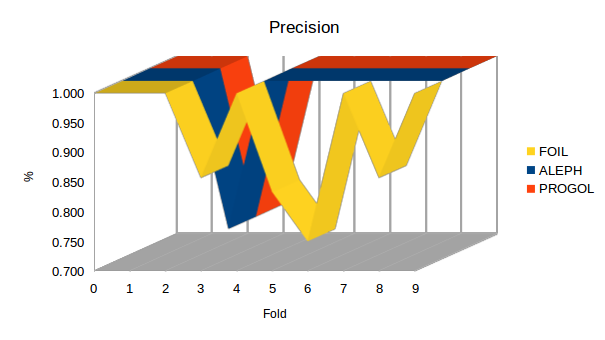
\includegraphics[width=1.2\textwidth]{img/datasetGraph/elsevier/precision.png}
	\label{Elsevier-Precision}
\end{figure}
\paragraph{Recall}
\begin{figure}[hbtp]
	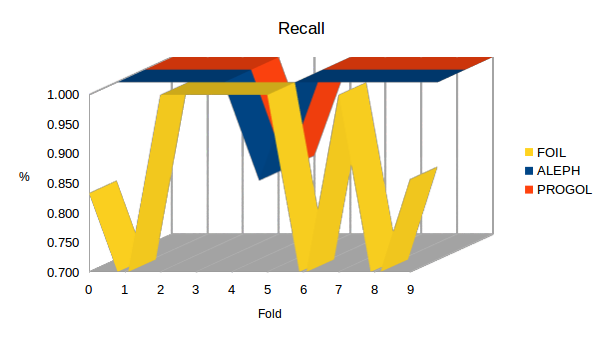
\includegraphics[width=1.2\textwidth]{img/datasetGraph/elsevier/recall.png}
	\label{Elsevier-Recall}
\end{figure}
\paragraph{F-Measure}
\begin{figure}[hbtp]
	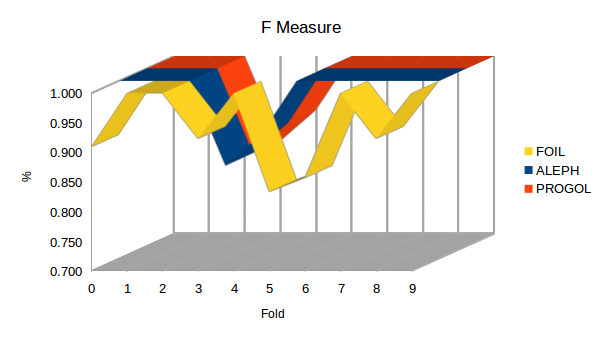
\includegraphics[width=1.2\textwidth]{img/datasetGraph/elsevier/fm.png}
	\label{Elsevier-F-measure}
\end{figure}
\paragraph{Accuracy}
\begin{figure}[hbtp]
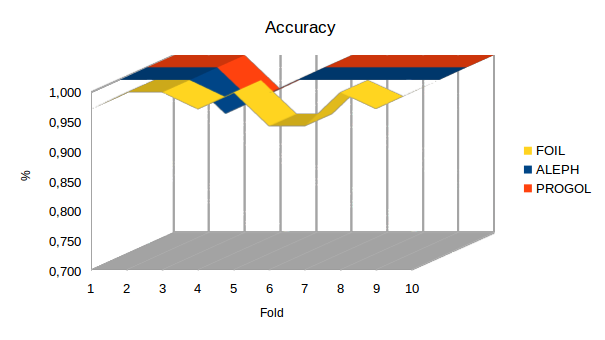
\includegraphics[width=1.2\textwidth]{img/datasetGraph/elsevier/accuracy.png}
\label{Elsevier-Accuracy}
\end{figure}
\paragraph{Error}
\begin{figure}[hbtp]
	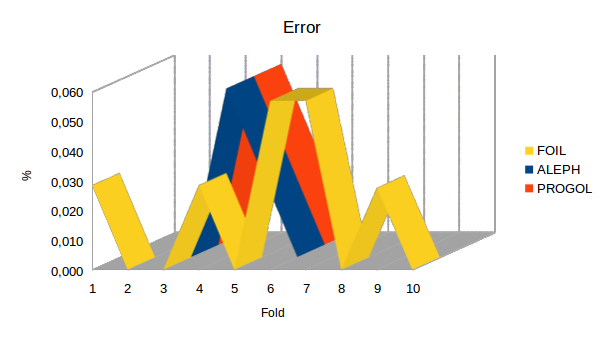
\includegraphics[width=1.2\textwidth]{img/datasetGraph/elsevier/error.png}
	\label{Elsevier-Error}
\end{figure}

\subsection{JMLR}
\subsubsection{ALEPH}
\pgfplotstabletypeset[
col sep=comma,
string type,
every head row/.style={%
	before row={\toprule\addlinespace
		%		\multicolumn{10}{c}{ALEPH}\\
	},
	after row=\addlinespace\midrule\addlinespace
},
every last row/.style={after row=\addlinespace\bottomrule},
columns/FOLD/.style={column name=FOLD, column type=c},
columns/TP/.style={column name=TP, column type=c},
columns/TN/.style={column name=TN, column type=c},
columns/FP/.style={column name=FP, column type=c},
columns/FN/.style={column name=FN, column type=c},
columns/precision/.style={column name=precision, column type=c},
columns/recall/.style={column name=recall, column type=c},
columns/F-Measure/.style={column name=F-Measure, column type=c},
columns/Acc/.style={column name=Accuracy, column type=c},
columns/Err/.style={column name=Error, column type=c},
]{csv/jmlr/aleph.csv}

\begin{verbatim}
jmlr started at 14:34:50
---Fold 0 started at 14:34:50
---Fold 0 ended in: 0:00:44.040336
---Fold 1 started at 14:35:34
---Fold 1 ended in: 0:00:58.375317
---Fold 2 started at 14:36:33
---Fold 2 ended in: 0:00:40.177290
---Fold 3 started at 14:37:13
---Fold 3 ended in: 0:00:31.072195
---Fold 4 started at 14:37:44
---Fold 4 ended in: 0:00:57.077835
---Fold 5 started at 14:38:41
---Fold 5 ended in: 0:00:58.648341
---Fold 6 started at 14:39:39
---Fold 6 ended in: 0:00:58.353248
---Fold 7 started at 14:40:38
---Fold 7 ended in: 0:00:58.888839
---Fold 8 started at 14:41:37
---Fold 8 ended in: 0:00:42.341782
---Fold 9 started at 14:42:19
---Fold 9 ended in: 0:00:43.150318
jmlr ended in 0:08:12.126228
\end{verbatim}
\subsubsection{PROGOL}
\pgfplotstabletypeset[
col sep=comma,
string type,
every head row/.style={%
	before row={\toprule\addlinespace
		%		\multicolumn{10}{c}{PROGOL}\\
	},
	after row=\addlinespace\midrule\addlinespace
},
every last row/.style={after row=\addlinespace\bottomrule},
columns/FOLD/.style={column name=FOLD, column type=c},
columns/TP/.style={column name=TP, column type=c},
columns/TN/.style={column name=TN, column type=c},
columns/FP/.style={column name=FP, column type=c},
columns/FN/.style={column name=FN, column type=c},
columns/precision/.style={column name=precision, column type=c},
columns/recall/.style={column name=recall, column type=c},
columns/F-Measure/.style={column name=F-Measure, column type=c},
columns/Acc/.style={column name=Accuracy, column type=c},
columns/Err/.style={column name=Error, column type=c},
]{csv/jmlr/progol.csv}

\begin{verbatim}
jmlr started at 09:29:44
---Fold 0 started at 09:29:44
---Fold 0 ended in: 0:00:26.084275
---Fold 1 started at 09:30:10
---Fold 1 ended in: 0:00:45.996500
---Fold 2 started at 09:30:56
---Fold 2 ended in: 0:00:37.654357
---Fold 3 started at 09:31:34
---Fold 3 ended in: 0:00:29.765864
---Fold 4 started at 09:32:04
---Fold 4 ended in: 0:00:41.809093
---Fold 5 started at 09:32:45
---Fold 5 ended in: 0:00:37.723421
---Fold 6 started at 09:33:23
---Fold 6 ended in: 0:00:19.029631
---Fold 7 started at 09:33:42
---Fold 7 ended in: 0:00:49.946552
---Fold 8 started at 09:34:32
---Fold 8 ended in: 0:00:34.581277
---Fold 9 started at 09:35:07
---Fold 9 ended in: 0:00:34.694070
jmlr ended in 0:05:57.285763
\end{verbatim}
\subsubsection{FOIL}
\pgfplotstabletypeset[
col sep=comma,
string type,
every head row/.style={%
	before row={\toprule\addlinespace
		%		\multicolumn{10}{c}{FOIL}\\
	},
	after row=\addlinespace\midrule\addlinespace
},
every last row/.style={after row=\addlinespace\bottomrule},
columns/FOLD/.style={column name=FOLD, column type=c},
columns/TP/.style={column name=TP, column type=c},
columns/TN/.style={column name=TN, column type=c},
columns/FP/.style={column name=FP, column type=c},
columns/FN/.style={column name=FN, column type=c},
columns/precision/.style={column name=precision, column type=c},
columns/recall/.style={column name=recall, column type=c},
columns/F-Measure/.style={column name=F-Measure, column type=c},
columns/Acc/.style={column name=Accuracy, column type=c},
columns/Err/.style={column name=Error, column type=c},
]{csv/jmlr/foil.csv}

\begin{verbatim}
jmlr started at 09:12:23
---Fold 0 started at 09:12:23
---Fold 0 ended in: 0:00:02.759541
---Fold 1 started at 09:12:26
---Fold 1 ended in: 0:00:05.639292
---Fold 2 started at 09:12:32
---Fold 2 ended in: 0:00:07.404179
---Fold 3 started at 09:12:39
---Fold 3 ended in: 0:00:03.042006
---Fold 4 started at 09:12:42
---Fold 4 ended in: 0:00:05.479597
---Fold 5 started at 09:12:48
---Fold 5 ended in: 0:00:03.189191
---Fold 6 started at 09:12:51
---Fold 6 ended in: 0:00:02.824482
---Fold 7 started at 09:12:54
---Fold 7 ended in: 0:00:02.231835
---Fold 8 started at 09:12:56
---Fold 8 ended in: 0:00:03.894108
---Fold 9 started at 09:13:00
---Fold 9 ended in: 0:00:03.966871
jmlr ended in 0:00:40.431931
\end{verbatim}
\subsubsection{Grafici}
\paragraph{Precision}
\begin{figure}[hbtp]
	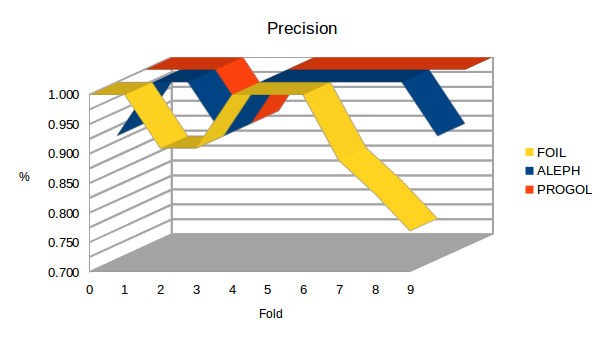
\includegraphics[width=1.2\textwidth]{img/datasetGraph/jmlr/precision.png}
	\label{JMLR-Precision}
\end{figure}
\paragraph{Recall}
\begin{figure}[hbtp]
	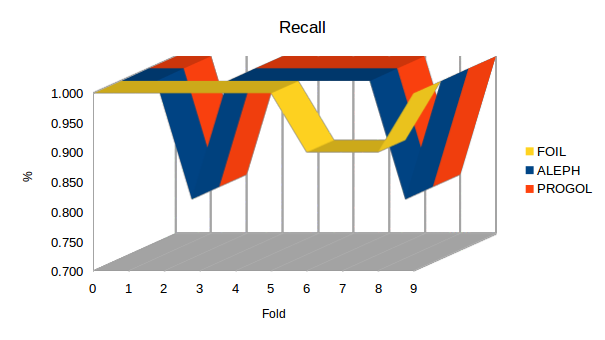
\includegraphics[width=1.2\textwidth]{img/datasetGraph/jmlr/recall.png}
	\label{JMLR-Recall}
\end{figure}
\paragraph{F-Measure}
\begin{figure}[hbtp]
	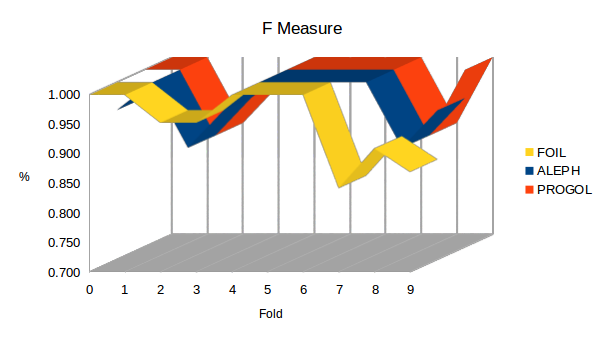
\includegraphics[width=1.2\textwidth]{img/datasetGraph/jmlr/fm.png}
	\label{JMLR-F-measure}
\end{figure}
\paragraph{Accuracy}
\begin{figure}[hbtp]
	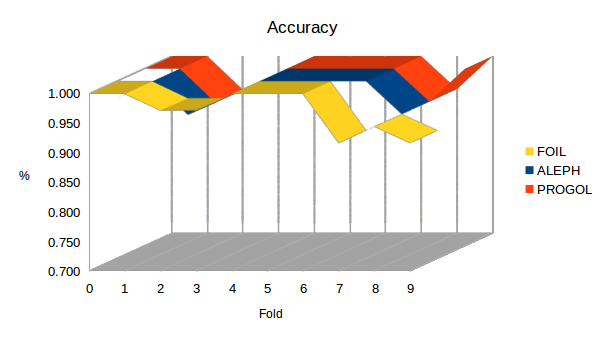
\includegraphics[width=1.2\textwidth]{img/datasetGraph/jmlr/accuracy.png}
	\label{JMLR-Accuracy}
\end{figure}
\paragraph{Error}
\begin{figure}[hbtp]
	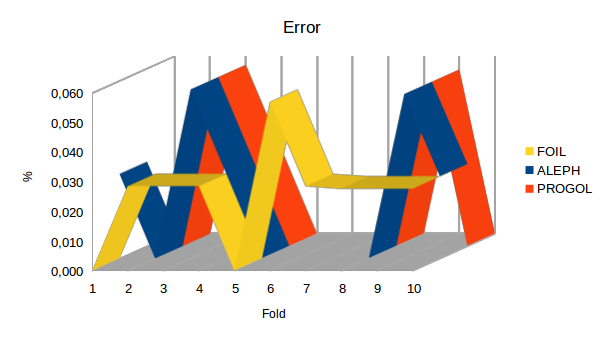
\includegraphics[width=1.2\textwidth]{img/datasetGraph/jmlr/error.png}
	\label{JMLR-Error}
\end{figure}

\subsection{SVLN}
\subsubsection{ALEPH}
\pgfplotstabletypeset[
col sep=comma,
string type,
every head row/.style={%
	before row={\toprule\addlinespace
		%		\multicolumn{10}{c}{ALEPH}\\
	},
	after row=\addlinespace\midrule\addlinespace
},
every last row/.style={after row=\addlinespace\bottomrule},
columns/FOLD/.style={column name=FOLD, column type=c},
columns/TP/.style={column name=TP, column type=c},
columns/TN/.style={column name=TN, column type=c},
columns/FP/.style={column name=FP, column type=c},
columns/FN/.style={column name=FN, column type=c},
columns/precision/.style={column name=precision, column type=c},
columns/recall/.style={column name=recall, column type=c},
columns/F-Measure/.style={column name=F-Measure, column type=c},
columns/Acc/.style={column name=Accuracy, column type=c},
columns/Err/.style={column name=Error, column type=c},
]{csv/svln/aleph.csv}

\begin{verbatim}
svln started at 18:53:32
---Fold 0 started at 18:53:32
---Fold 0 ended in: 0:01:54.234807
---Fold 1 started at 18:55:26
---Fold 1 ended in: 0:01:35.397646
---Fold 2 started at 18:57:02
---Fold 2 ended in: 0:01:43.559253
---Fold 3 started at 18:58:45
---Fold 3 ended in: 0:01:52.177093
---Fold 4 started at 19:00:38
---Fold 4 ended in: 0:02:31.127063
---Fold 5 started at 19:03:09
---Fold 5 ended in: 0:01:47.824715
---Fold 6 started at 19:04:56
---Fold 6 ended in: 0:01:40.269009
---Fold 7 started at 19:06:37
---Fold 7 ended in: 0:01:15.299631
---Fold 8 started at 19:07:52
---Fold 8 ended in: 0:01:39.995804
---Fold 9 started at 19:09:32
---Fold 9 ended in: 0:02:01.367264
svln ended in 0:18:01.252851
\end{verbatim}
\subsubsection{PROGOL}
\pgfplotstabletypeset[
col sep=comma,
string type,
every head row/.style={%
	before row={\toprule\addlinespace
		%		\multicolumn{10}{c}{PROGOL}\\
	},
	after row=\addlinespace\midrule\addlinespace
},
every last row/.style={after row=\addlinespace\bottomrule},
columns/FOLD/.style={column name=FOLD, column type=c},
columns/TP/.style={column name=TP, column type=c},
columns/TN/.style={column name=TN, column type=c},
columns/FP/.style={column name=FP, column type=c},
columns/FN/.style={column name=FN, column type=c},
columns/precision/.style={column name=precision, column type=c},
columns/recall/.style={column name=recall, column type=c},
columns/F-Measure/.style={column name=F-Measure, column type=c},
columns/Acc/.style={column name=Accuracy, column type=c},
columns/Err/.style={column name=Error, column type=c},
]{csv/svln/progol.csv}

\begin{verbatim}
	svln started at 12:43:51
	---Fold 0 started at 12:43:51
	---Fold 0 ended in: 0:01:04.320244
	---Fold 1 started at 12:44:55
	---Fold 1 ended in: 0:01:24.453421
	---Fold 2 started at 12:46:20
	---Fold 2 ended in: 0:01:12.648375
	---Fold 3 started at 12:47:32
	---Fold 3 ended in: 0:01:00.633611
	---Fold 4 started at 12:48:33
	---Fold 4 ended in: 0:01:18.982588
	---Fold 5 started at 12:49:52
	---Fold 5 ended in: 0:01:16.183743
	---Fold 6 started at 12:51:08
	---Fold 6 ended in: 0:01:00.154165
	---Fold 7 started at 12:52:08
	---Fold 7 ended in: 0:00:42.924736
	---Fold 8 started at 12:52:51
	---Fold 8 ended in: 0:01:24.184806
	---Fold 9 started at 12:54:15
	---Fold 9 ended in: 0:01:44.461413
	svln ended in 0:12:08.991536
\end{verbatim}
\subsubsection{FOIL}
\pgfplotstabletypeset[
col sep=comma,
string type,
every head row/.style={%
	before row={\toprule\addlinespace
		%		\multicolumn{10}{c}{FOIL}\\
	},
	after row=\addlinespace\midrule\addlinespace
},
every last row/.style={after row=\addlinespace\bottomrule},
columns/FOLD/.style={column name=FOLD, column type=c},
columns/TP/.style={column name=TP, column type=c},
columns/TN/.style={column name=TN, column type=c},
columns/FP/.style={column name=FP, column type=c},
columns/FN/.style={column name=FN, column type=c},
columns/precision/.style={column name=precision, column type=c},
columns/recall/.style={column name=recall, column type=c},
columns/F-Measure/.style={column name=F-Measure, column type=c},
columns/Acc/.style={column name=Accuracy, column type=c},
columns/Err/.style={column name=Error, column type=c},
]{csv/svln/foil.csv}

\begin{verbatim}
svln started at 09:13:04
---Fold 0 started at 09:13:04
---Fold 0 ended in: 0:00:00.328284
---Fold 1 started at 09:13:04
---Fold 1 ended in: 0:00:00.238981
---Fold 2 started at 09:13:05
---Fold 2 ended in: 0:00:00.294530
---Fold 3 started at 09:13:05
---Fold 3 ended in: 0:00:00.207063
---Fold 4 started at 09:13:05
---Fold 4 ended in: 0:00:00.242937
---Fold 5 started at 09:13:05
---Fold 5 ended in: 0:00:00.191957
---Fold 6 started at 09:13:06
---Fold 6 ended in: 0:00:00.194648
---Fold 7 started at 09:13:06
---Fold 7 ended in: 0:00:00.340427
---Fold 8 started at 09:13:06
---Fold 8 ended in: 0:00:00.318204
---Fold 9 started at 09:13:06
---Fold 9 ended in: 0:00:00.208281
svln ended in 0:00:02.566150
\end{verbatim}

\subsubsection{Grafici}
\paragraph{Precision}
\begin{figure}[hbtp]
	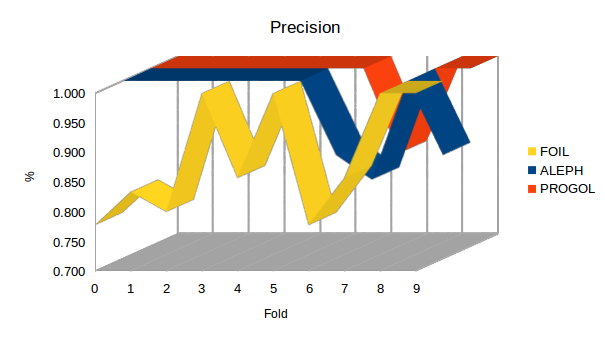
\includegraphics[width=1.2\textwidth]{img/datasetGraph/svln/precision.png}
	\label{svln-Precision}
\end{figure}
\paragraph{Recall}
\begin{figure}[hbtp]
	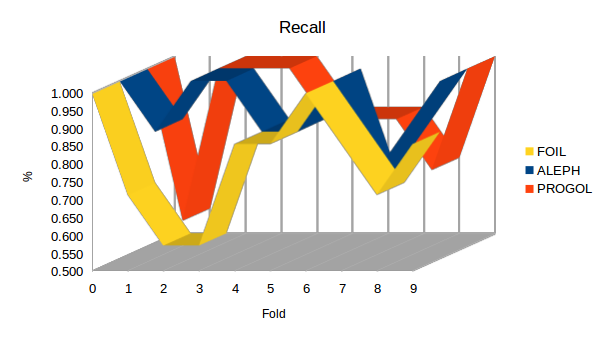
\includegraphics[width=1.2\textwidth]{img/datasetGraph/svln/recall.png}
	\label{svln-Recall}
\end{figure}
\paragraph{F-Measure}
\begin{figure}[hbtp]
	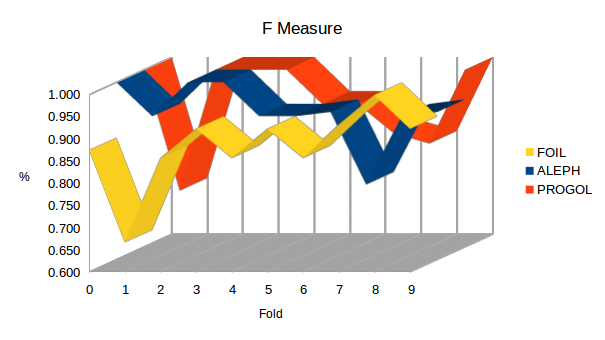
\includegraphics[width=1.2\textwidth]{img/datasetGraph/svln/fm.png}
	\label{svln-F-measure}
\end{figure}
\paragraph{Accuracy}
\begin{figure}[hbtp]
	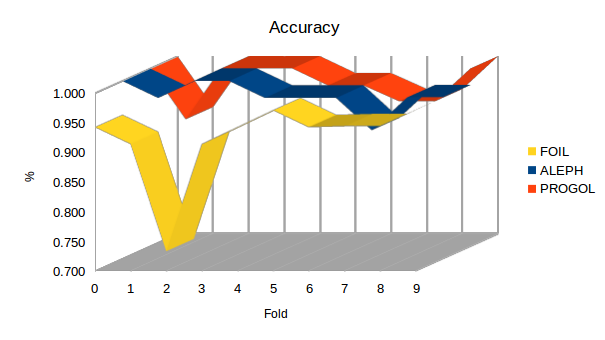
\includegraphics[width=1.2\textwidth]{img/datasetGraph/svln/accuracy.png}
	\label{svln-Accuracy}
\end{figure}
\paragraph{Error}
\begin{figure}[hbtp]
	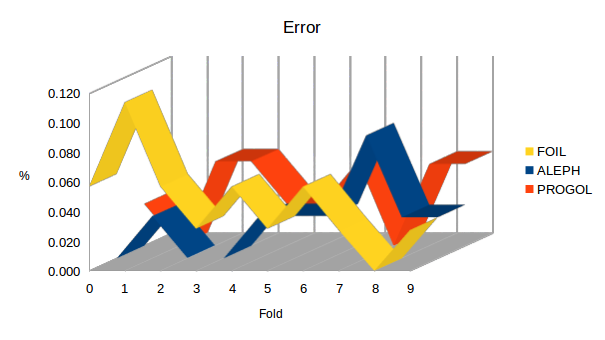
\includegraphics[width=1.2\textwidth]{img/datasetGraph/svln/error.png}
	\label{svln-Error}
\end{figure}

\subsection{MLJ - discretizzato}
\subsubsection{ALEPH}
\pgfplotstabletypeset[
col sep=comma,
string type,
every head row/.style={%
	before row={\toprule\addlinespace
		%		\multicolumn{10}{c}{ALEPH}\\
	},
	after row=\addlinespace\midrule\addlinespace
},
every last row/.style={after row=\addlinespace\bottomrule},
columns/FOLD/.style={column name=FOLD, column type=c},
columns/TP/.style={column name=TP, column type=c},
columns/TN/.style={column name=TN, column type=c},
columns/FP/.style={column name=FP, column type=c},
columns/FN/.style={column name=FN, column type=c},
columns/precision/.style={column name=precision, column type=c},
columns/recall/.style={column name=recall, column type=c},
columns/F-Measure/.style={column name=F-Measure, column type=c},
columns/Acc/.style={column name=Accuracy, column type=c},
columns/Err/.style={column name=Error, column type=c},
]{csv/mlj/discr/aleph.csv}

\begin{verbatim}
mlj discr started at 12:38:52
---Fold 0 started at 12:38:52
---Fold 0 ended in: 0:06:32.987887
---Fold 1 started at 12:45:25
---Fold 1 ended in: 0:06:55.407367
---Fold 2 started at 12:52:20
---Fold 2 ended in: 0:06:38.581722
---Fold 3 started at 12:58:59
---Fold 3 ended in: 0:06:40.096561
---Fold 4 started at 13:05:39
---Fold 4 ended in: 0:06:42.671273
---Fold 5 started at 13:12:22
---Fold 5 ended in: 0:06:46.315155
---Fold 6 started at 13:19:08
---Fold 6 ended in: 0:06:29.094981
---Fold 7 started at 13:25:37
---Fold 7 ended in: 0:06:49.495072
---Fold 8 started at 13:32:26
---Fold 8 ended in: 0:05:32.322452
---Fold 9 started at 13:37:59
---Fold 9 ended in: 0:05:26.615672
mlj discr ended in 1:04:33.588808
\end{verbatim}

\subsubsection{PROGOL}
\pgfplotstabletypeset[
col sep=comma,
string type,
every head row/.style={%
	before row={\toprule\addlinespace
		%		\multicolumn{10}{c}{PROGOL}\\
	},
	after row=\addlinespace\midrule\addlinespace
},
every last row/.style={after row=\addlinespace\bottomrule},
columns/FOLD/.style={column name=FOLD, column type=c},
columns/TP/.style={column name=TP, column type=c},
columns/TN/.style={column name=TN, column type=c},
columns/FP/.style={column name=FP, column type=c},
columns/FN/.style={column name=FN, column type=c},
columns/precision/.style={column name=precision, column type=c},
columns/recall/.style={column name=recall, column type=c},
columns/F-Measure/.style={column name=F-Measure, column type=c},
columns/Acc/.style={column name=Accuracy, column type=c},
columns/Err/.style={column name=Error, column type=c},
]{csv/mlj/discr/progol.csv}

\begin{verbatim}
mlj discr started at 14:35:28
---Fold 0 started at 14:35:28
---Fold 0 ended in: 0:05:33.172855
---Fold 1 started at 14:41:01
---Fold 1 ended in: 0:04:24.460047
---Fold 2 started at 14:45:25
---Fold 2 ended in: 0:06:21.096485
---Fold 3 started at 14:51:46
---Fold 3 ended in: 0:04:39.550606
---Fold 4 started at 14:56:26
---Fold 4 ended in: 0:05:39.287544
---Fold 5 started at 15:02:05
---Fold 5 ended in: 0:04:42.005965
---Fold 6 started at 15:06:47
---Fold 6 ended in: 0:05:36.268812
---Fold 7 started at 15:12:23
---Fold 7 ended in: 0:05:15.292060
---Fold 8 started at 15:17:39
---Fold 8 ended in: 0:04:34.640609
---Fold 9 started at 15:22:13
---Fold 9 ended in: 0:04:57.705908
mlj discr ended in 0:51:43.481549
\end{verbatim}
\subsubsection{FOIL}
\pgfplotstabletypeset[
col sep=comma,
string type,
every head row/.style={%
	before row={\toprule\addlinespace
		%		\multicolumn{10}{c}{FOIL}\\
	},
	after row=\addlinespace\midrule\addlinespace
},
every last row/.style={after row=\addlinespace\bottomrule},
columns/FOLD/.style={column name=FOLD, column type=c},
columns/TP/.style={column name=TP, column type=c},
columns/TN/.style={column name=TN, column type=c},
columns/FP/.style={column name=FP, column type=c},
columns/FN/.style={column name=FN, column type=c},
columns/precision/.style={column name=precision, column type=c},
columns/recall/.style={column name=recall, column type=c},
columns/F-Measure/.style={column name=F-Measure, column type=c},
columns/Acc/.style={column name=Accuracy, column type=c},
columns/Err/.style={column name=Error, column type=c},
]{csv/mlj/discr/foil.csv}

\begin{verbatim}
mlj discr started at 11:59:39
---Fold 0 started at 11:59:39
---Fold 0 ended in: 0:00:00.224591
---Fold 1 started at 11:59:40
---Fold 1 ended in: 0:00:00.237705
---Fold 2 started at 11:59:40
---Fold 2 ended in: 0:00:00.231943
---Fold 3 started at 11:59:40
---Fold 3 ended in: 0:00:00.225304
---Fold 4 started at 11:59:40
---Fold 4 ended in: 0:00:00.269991
---Fold 5 started at 11:59:41
---Fold 5 ended in: 0:00:00.227715
---Fold 6 started at 11:59:41
---Fold 6 ended in: 0:00:00.215050
---Fold 7 started at 11:59:41
---Fold 7 ended in: 0:00:00.271112
---Fold 8 started at 11:59:41
---Fold 8 ended in: 0:00:00.182183
---Fold 9 started at 11:59:42
---Fold 9 ended in: 0:00:00.206913
mlj discr ended in 0:00:02.293352
\end{verbatim}

\subsubsection{Grafici}
\paragraph{Precision}
\begin{figure}[hbtp]
	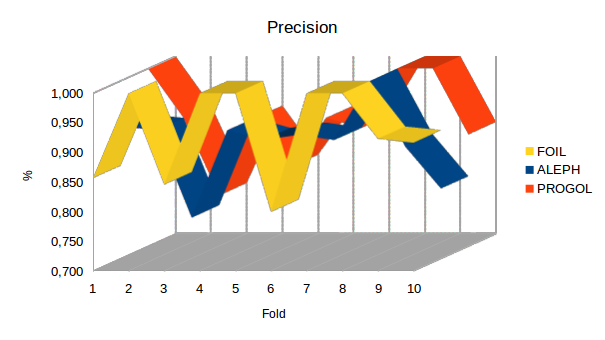
\includegraphics[width=1.2\textwidth]{img/datasetGraph/mlj/discr/precision.png}
	\label{mljdiscr-Precision}
\end{figure}
\paragraph{Recall}
\begin{figure}[hbtp]
	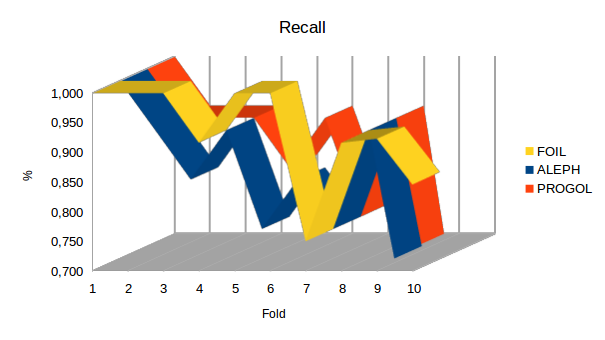
\includegraphics[width=1.2\textwidth]{img/datasetGraph/mlj/discr/recall.png}
	\label{mljdiscr-Recall}
\end{figure}
\paragraph{F-Measure}
\begin{figure}[hbtp]
	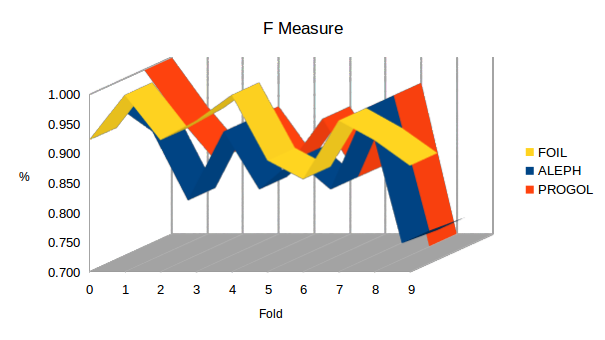
\includegraphics[width=1.2\textwidth]{img/datasetGraph/mlj/discr/fm.png}
	\label{mljdiscr-F-measure}
\end{figure}
\paragraph{Accuracy}
\begin{figure}[hbtp]
	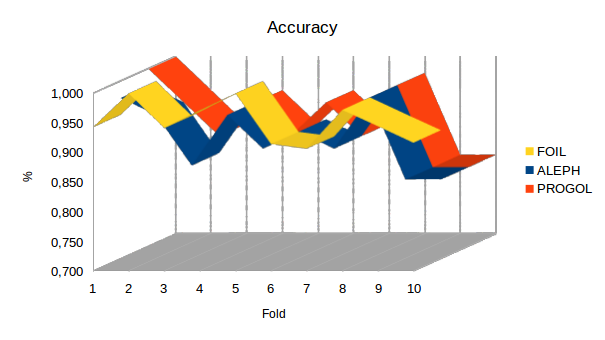
\includegraphics[width=1.2\textwidth]{img/datasetGraph/mlj/discr/accuracy.png}
	\label{mljdiscr-Accuracy}
\end{figure}
\paragraph{Error}
\begin{figure}[hbtp]
	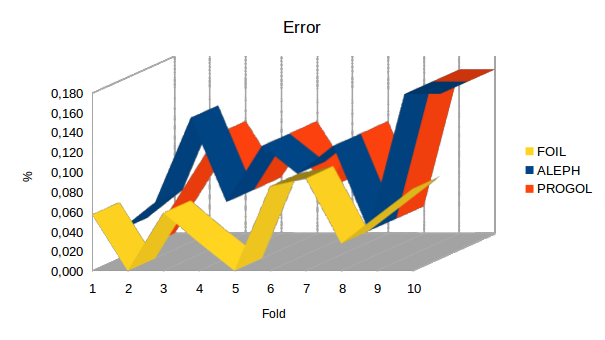
\includegraphics[width=1.2\textwidth]{img/datasetGraph/mlj/discr/error.png}
	\label{mljdiscr-Error}
\end{figure}

\subsection{MLJ - non discretizzato}
\subsubsection{ALEPH}
\pgfplotstabletypeset[
col sep=comma,
string type,
every head row/.style={%
	before row={\toprule\addlinespace
		%		\multicolumn{10}{c}{ALEPH}\\
	},
	after row=\addlinespace\midrule\addlinespace
},
every last row/.style={after row=\addlinespace\bottomrule},
columns/FOLD/.style={column name=FOLD, column type=c},
columns/TP/.style={column name=TP, column type=c},
columns/TN/.style={column name=TN, column type=c},
columns/FP/.style={column name=FP, column type=c},
columns/FN/.style={column name=FN, column type=c},
columns/precision/.style={column name=precision, column type=c},
columns/recall/.style={column name=recall, column type=c},
columns/F-Measure/.style={column name=F-Measure, column type=c},
columns/Acc/.style={column name=Accuracy, column type=c},
columns/Err/.style={column name=Error, column type=c},
]{csv/mlj/nodiscr/aleph.csv}

\begin{verbatim}
mlj nodiscr started at 13:57:41
---Fold 0 started at 13:57:41
---Fold 0 ended in: 0:02:21.787734
---Fold 1 started at 14:00:03
---Fold 1 ended in: 0:04:07.386826
---Fold 2 started at 14:04:10
---Fold 2 ended in: 0:04:17.316495
---Fold 3 started at 14:08:27
---Fold 3 ended in: 0:04:06.532924
---Fold 4 started at 14:12:34
---Fold 4 ended in: 0:04:10.948141
---Fold 5 started at 14:16:45
---Fold 5 ended in: 0:04:06.952672
---Fold 6 started at 14:20:52
---Fold 6 ended in: 0:04:48.798386
---Fold 7 started at 14:25:41
---Fold 7 ended in: 0:04:43.446125
---Fold 8 started at 14:30:24
---Fold 8 ended in: 0:08:46.085098
---Fold 9 started at 14:39:10
---Fold 9 ended in: 0:05:54.209124
mlj nodiscr ended in 0:47:23.464204
\end{verbatim}

\subsubsection{PROGOL}
\pgfplotstabletypeset[
col sep=comma,
string type,
every head row/.style={%
	before row={\toprule\addlinespace
		%		\multicolumn{10}{c}{PROGOL}\\
	},
	after row=\addlinespace\midrule\addlinespace
},
every last row/.style={after row=\addlinespace\bottomrule},
columns/FOLD/.style={column name=FOLD, column type=c},
columns/TP/.style={column name=TP, column type=c},
columns/TN/.style={column name=TN, column type=c},
columns/FP/.style={column name=FP, column type=c},
columns/FN/.style={column name=FN, column type=c},
columns/precision/.style={column name=precision, column type=c},
columns/recall/.style={column name=recall, column type=c},
columns/F-Measure/.style={column name=F-Measure, column type=c},
columns/Acc/.style={column name=Accuracy, column type=c},
columns/Err/.style={column name=Error, column type=c},
]{csv/mlj/nodiscr/progol.csv}

\begin{verbatim}
mlj nodiscr started at 15:13:39
---Fold 0 started at 15:13:39
---Fold 0 ended in: 0:01:56.835496
---Fold 1 started at 15:15:36
---Fold 1 ended in: 0:03:59.207766
---Fold 2 started at 15:19:35
---Fold 2 ended in: 0:05:05.807433
---Fold 3 started at 15:24:41
---Fold 3 ended in: 0:06:07.573072
---Fold 4 started at 15:30:48
---Fold 4 ended in: 0:02:00.128641
---Fold 5 started at 15:32:48
---Fold 5 ended in: 0:06:00.366362
---Fold 6 started at 15:38:49
---Fold 6 ended in: 0:03:54.306654
---Fold 7 started at 15:42:43
---Fold 7 ended in: 0:04:42.558320
---Fold 8 started at 15:47:26
---Fold 8 ended in: 0:02:21.500061
---Fold 9 started at 15:49:47
---Fold 9 ended in: 0:02:10.637707
mlj nodiscr ended in 0:38:18.922015
\end{verbatim}
\subsubsection{FOIL}

\pgfplotstabletypeset[
col sep=comma,
string type,
every head row/.style={%
	before row={\toprule\addlinespace
		%		\multicolumn{10}{c}{FOIL}\\
	},
	after row=\addlinespace\midrule\addlinespace
},
every last row/.style={after row=\addlinespace\bottomrule},
columns/FOLD/.style={column name=FOLD, column type=c},
columns/TP/.style={column name=TP, column type=c},
columns/TN/.style={column name=TN, column type=c},
columns/FP/.style={column name=FP, column type=c},
columns/FN/.style={column name=FN, column type=c},
columns/precision/.style={column name=precision, column type=c},
columns/recall/.style={column name=recall, column type=c},
columns/F-Measure/.style={column name=F-Measure, column type=c},
columns/Acc/.style={column name=Accuracy, column type=c},
columns/Err/.style={column name=Error, column type=c}
]{csv/mlj/nodiscr/foil.csv}

\begin{verbatim}
mlj nodiscr started at 13:48:52
---Fold 0 started at 13:48:52
---Fold 0 ended in: 0:00:02.204258
---Fold 1 started at 13:48:55
---Fold 1 ended in: 0:00:26.650516
---Fold 2 started at 13:49:21
---Fold 2 ended in: 0:00:26.171711
---Fold 3 started at 13:49:47
---Fold 3 ended in: 0:00:46.732210
---Fold 4 started at 13:50:34
---Fold 4 ended in: 0:00:51.158960
---Fold 5 started at 13:51:25
---Fold 5 ended in: 0:00:05.917821
---Fold 6 started at 13:51:31
---Fold 6 ended in: 0:00:23.688156
---Fold 7 started at 13:51:55
---Fold 7 ended in: 0:00:28.056554
---Fold 8 started at 13:52:23
---Fold 8 ended in: 0:00:51.933317
---Fold 9 started at 13:53:15
---Fold 9 ended in: 0:00:06.915890
mlj nodiscr ended in 0:04:29.430078
\end{verbatim}

\subsubsection{Grafici}
\paragraph{Precision}
\begin{figure}[hbtp]
	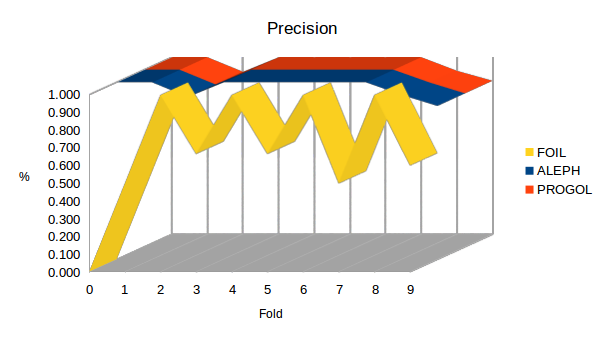
\includegraphics[width=1.2\textwidth]{img/datasetGraph/mlj/nodiscr/precision.png}
	\label{mljnodiscr-Precision}
\end{figure}
\paragraph{Recall}
\begin{figure}[hbtp]
	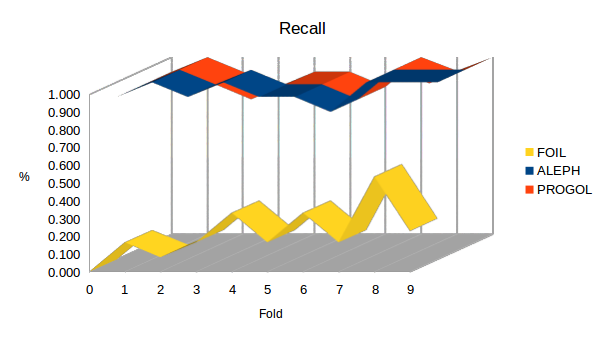
\includegraphics[width=1.2\textwidth]{img/datasetGraph/mlj/nodiscr/recall.png}
	\label{mljnodiscr-Recall}
\end{figure}
\paragraph{F-Measure}
\begin{figure}[hbtp]
	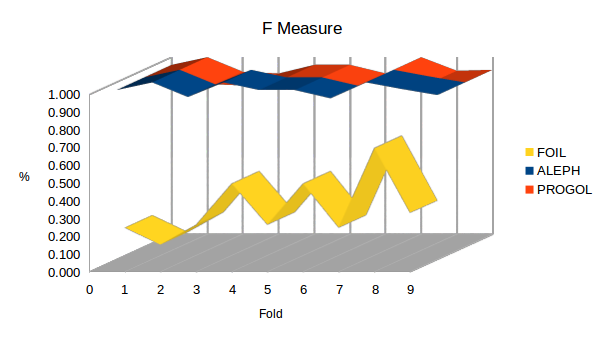
\includegraphics[width=1.2\textwidth]{img/datasetGraph/mlj/nodiscr/fm.png}
	\label{mljnodiscr-F-measure}
\end{figure}
\paragraph{Accuracy}
\begin{figure}[hbtp]
	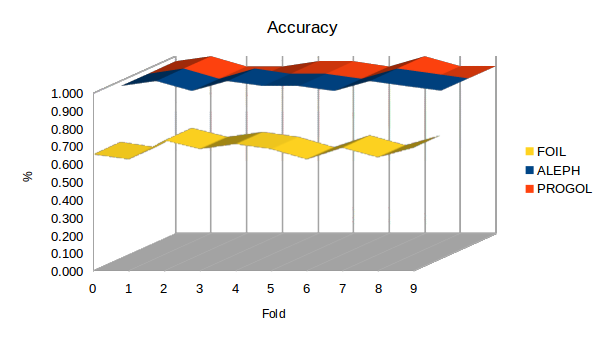
\includegraphics[width=1.2\textwidth]{img/datasetGraph/mlj/nodiscr/accuracy.png}
	\label{mljnodiscr-Accuracy}
\end{figure}
\paragraph{Error}
\begin{figure}[hbtp]
	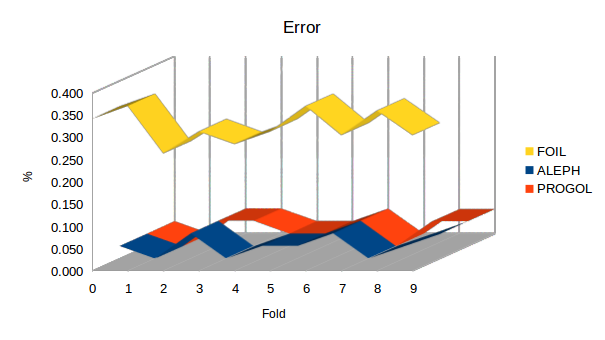
\includegraphics[width=1.2\textwidth]{img/datasetGraph/mlj/nodiscr/error.png}
	\label{mljnodiscr-Error}
\end{figure}
\section{Test di Valutazione}
\nocite{friedmanTest}
\nocite{wiki:Friedman}
Per poter analizzare i dati da un punto di vista statistico in modo da capire quale dei tre sistemi risulti essere migliore in un task di classificazione, è necessario utilizzare un test delle ipotesi che sia in grado di rigettare o confermare l'ipotesi nulla.

L'ipotesi nulla da rigettare in particolare sarà:
$$H_0 : \mu_{ALEPH} = \mu_{PROGOL} = \mu_{FOIL} $$
Mentre, l'ipotesi alternativa da accettare sarà:
$$H_1 : \mu_{ALEPH} \neq \mu_{PROGOL} \neq \mu_{FOIL} $$

Tra le diverse metriche calcolate per i diversi algoritmi, l'accuratezza è la metrica utilizzata affinché venga verificato il test delle ipotesi.

Poiché per ogni dataset è stata ripetuta la sperimentazione, il test delle ipotesi sarà condotto per ognuno dei cinque dataset separatamente.
Il test da effettuare dovrà rispettare i seguenti vincoli dettati dal dataset e dal tipo di sperimentazione che è stata effettuata:
\begin{itemize}
	\item \textbf{Numero di campioni maggiore di due}: Visto il quantitativo di campioni da analizzare, il test da scegliere dovrà essere in grado di processare un numero di campioni pari a tre.
	\item \textbf{Dimensione del campione limitata}: Dato che il valore dell'accuratezza è stata calcolata per ogni fold, il dimensione del campione sarà limitato a dieci, nonché il numero di fold creati. Questo fa si che il test da scegliere dovrà essere necessariamente un tipo di test non parametrico in quanto, visto l'esiguo quantitativo di elementi, non può essere garantita nè la omoschedasticità, nè che i gruppi dei dati appartengano ad una popolazione con distribuzione normale.
	\item \textbf{Campioni dipendenti}: a causa dell'utilizzo della tecnica della k-fold cross validation i sistemi sono stati analizzati utilizzando gli stessi identici fold, rendendo cosi dipendenti i campioni.
\end{itemize}

Visti i requisiti che il test dovrà rispettare, il test scelto per la verifica delle ipotesi è il Friedman test, il quale è un test non parametrico utilizzato per testare la differenza tra i diversi campioni correlati.
L'ipotesi nulla del test di Friedman è che non ci sia differenza significativa tra le variabili. Se la probabilità calcolata è bassa (P è inferiore al livello di significatività selezionato) l'ipotesi nulla verrà rigettata e si potrà concludere che almeno due delle variabili sono significativamente differenti con le altre.

Si è deciso di utilizzare un livello di significatività $\alpha$ pari al 5\%.

Per calcolare questo tipo di test è stato utilizzato un software atto a realizzare test statistici quale MedCalc \textcopyright.
Di seguito verrà mostrato un esempio di output restituito dal programma, in particolare, ciò che è stato restituito dal confronto tra i tre sistemi sul dataset MLJ discretizzato:
\begin{figure}[H]
	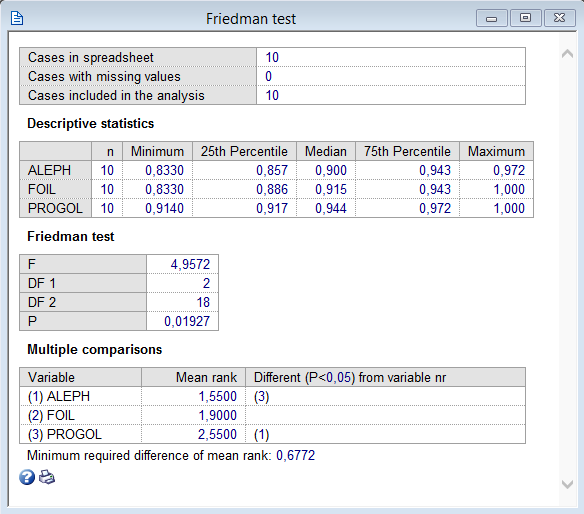
\includegraphics[width=0.9\textwidth]{img/TestResult/mljdiscr.png}
	\label{Friedman Test - MLJ Discretizzato}
\end{figure}

Riepilogando i risultati dei vari test statistici si evince che:

\begin{lstlisting}
     $\mu$        ALEPH   PROGOL  FOIL   P-Value     $H_0$
     
Elsevier       1       1     0,972  0.05346   Rigettata
JMLR         0.986     1     0.986  0.60765   Accettata
MLJ Disc     0.9     0.915   0.944  0.01927   Rigettata
MLJ No Disc  0,971   0.958   0.686  0.00001   Rigettata
SVLN         0.972   0.986   0.957  0.12942   Accettata
\end{lstlisting}


Inoltre, con questo test è possibile anche individuare le coppie che hanno portato a rigettare l'ipotesi nulla. Nel nostro caso le coppie che hanno portato a rigettare l'ipotesi nulla sono state:

\begin{itemize}
	\item Elsevier:
		\begin{itemize}
			\item Aleph - Foil
			\item Progol - Foil
		\end{itemize}
	\item MLJ non discretizzato:
		\begin{itemize}
			\item Aleph - Foil
			\item Aleph - Progol
			\item Foil - Progol
		\end{itemize}
	\item MLJ discretizzato:
		\begin{itemize}
			\item Aleph - Foil
		\end{itemize}
\end{itemize}

%\section{Test di ValutazioneOLD}
%Per poter analizzare i dati da un punto di vista statistico in modo da capire quale dei tre sistemi risulti essere migliore in un task di classificazione, è necessario utilizzare un test delle ipotesi che sia in grado di rigettare o confermare l'ipotesi nulla.
%
%L'ipotesi nulla da rigettare in particolare sarà:
%$$H_0 : \mu_{ALEPH} = \mu_{PROGOL} = \mu_{FOIL} $$
%Simmetricamente l'ipotesi alternativa sarà:
%$$H_1 : \mu_{ALEPH} \neq \mu_{PROGOL} \neq \mu_{FOIL} $$
%
%Tra le diverse metriche calcolate per i diversi algoritmi, l'accuratezza è la metrica utilizzata affinché venga verificato il test delle ipotesi.
%
%Poiché per ogni dataset è stata ripetuta la sperimentazione, il test delle ipotesi sarà condotto per ognuno dei cinque dataset separatamente.
%
%Considerato il numero di sistemi da confrontare, il test più adatto per verificare questo tipo di ipotesi è il test parametrico ANOVA (\textbf{AN}alysis \textbf{O}f \textbf{VA}riance). Questo test presuppone che i gruppi di dati provengano da una popolazione normale in ipotesi di omoschedasticità (ossia, la varianza dei gruppi è la stessa di quella della popolazione),condizione veritiera nei dataset a disposizione. 
%
%Si è deciso di usare un livello $\alpha$ di soglia pari al 5\%.
%
%Attraverso l'ausilio di un foglio di calcolo costruito ad-hoc, sono stati estratti i risultati del test, di seguito un sunto di ciò che si è ottenuto.
%
%\begin{verbatim}
%Elsevier
%
%               ALEPH   PROGOL   FOIL
%      $\mu$    0,99     0,99    0,97       Livello \alpha    0,05
%   $\sigma$    0,02     0,02    0,03       Quantile Teorico  3,35
%     
%  Consuntivo   3,66
%                               H0 rigettato
%\end{verbatim}
%
%\begin{verbatim}
%JMLR
%
%               ALEPH   PROGOL   FOIL
%      $\mu$    0,98     0,99    0,97       Livello \alpha    0,05
%   $\sigma$    0,02     0,02    0,03       Quantile Teorico  3,35
%     
%  Consuntivo   0,74
%                               H0 accettato
%\end{verbatim}
%
%\begin{verbatim}
%MLJ - Non discretizzato
%
%               ALEPH   PROGOL   FOIL
%      $\mu$    0,97     0,96    0,71       Livello \alpha    0,05
%   $\sigma$    0,02     0,02    0,06       Quantile Teorico  3,35
%     
%  Consuntivo   138,92
%                               H0 rigettato
%\end{verbatim}
%
%\begin{verbatim}
%MLJ - Discretizzato
%
%               ALEPH   PROGOL   FOIL
%      $\mu$    0,9     0,91    0,95       Livello \alpha    0,05
%   $\sigma$    0,05     0,06    0,03       Quantile Teorico  3,35
%     
%  Consuntivo   3,47
%                               H0 rigettato
%\end{verbatim}
%
%\begin{verbatim}
%SVLN
%               ALEPH   PROGOL   FOIL
%      $\mu$    0,97     0,97    0,95       Livello \alpha    0,05
%   $\sigma$    0,02     0,03    0,03       Quantile Teorico  3,35
%     
%  Consuntivo   1,70
%                               H0 accettato
%\end{verbatim}

%Analizzando i risultati cosi ottenuti, si evince che solo in due dei quattro dataset (JMLR e SVLN), i tre algoritmi risultano essere statisticamente uguali in termini di accuratezza predittiva.
\section{Conclusioni}

In questo documento sono stati confrontati tre sistemi di apprendimento su un task di classificazione binaria di layout di documenti testuali.

I dataset presi in considerazione sono stati quattro, ai quali è stato aggiunto un quinto generato dalla rappresentazione discretizzata su alcuni valori numerici di uno dei precedenti quattro. Ogni dataset è stato suddiviso in 10 fold, secondo uno schema di campionamento casuale stratificato.

I risultati mostrano una sostanziale similarità tra ALEPH e Progol su tutti i dataset. 
FOIL invece, pur evidenziando le migliori prestazioni in termini di tempo, 

Il test statistico

\clearpage

\appendix
\appendixpage
\addappheadtotoc
\section{Suddivisione in fold}
\label{appendix:fold}
Allo scopo di garantire la replicabilità degli esperimenti, riportiamo l'esatta suddivisione in fold dei 4 dataset.

Il segno +/- davanti all'id del documento indica che si tratta di un esempio positivo/negativo in quel dataset.

Il rapporto tra esempi positivi ed esempi negativi all'interno di ciascun fold rispecchia il rapporto esistente nel dataset intero, poiché realizzati per mezzo di un campionamento casuale stratificato.

\scriptsize
\begin{multicols}{4}
\subsection{elsevier}
\vspace{.5cm}

\subsubsection*{Fold0}
+sciserv45\\
+sciserv47\\
+sciserv46\\
+sciserv48\\
+sciserv8\\
+d06090909534026371\\
-d37290944\\
-d37290461\\
-d06060510413614235\\
-d06060518265400597\\
-d06053013393813816\\
-ong05a\\
-passerini06a\\
-d06060518540302460\\
-d06053013403113871\\
-d06053013250012940\\
-d06053013422814008\\
-d06060518310700907\\
-d37290308\\
-osborne02a\\
-d06053013252512990\\
-d06060518313100932\\
-forman03a\\
-d06060518272200636\\
-d37291002\\
-d37290816\\
-d06060518303100860\\
-d06060518492902207\\
-d06060510434514330\\
-spratling06a\\
-d06053013245412933\\
-jebara04a\\
-ling02a\\
-d37290745\\
-d37290186\\
\subsubsection*{Fold1}
+sciserv37\\
+sciserv6\\
+sciserv28\\
+sciserv21\\
+sciserv36\\
+sciserv27\\
-d06060518251800523\\
-demsar06a\\
-d06060518541902465\\
-manevitz01a\\
-d37290082\\
-botta03a\\
-d06060518383601440\\
-d37290491\\
-jaeger05a\\
-d06053013401813843\\
-d06060518532502449\\
-almeida05a\\
-d06060518284000724\\
-d06053013254713021\\
-d06053013251312977\\
-d37290232\\
-boulle05a\\
-d37290928\\
-d06060518433401633\\
-ryabko06a\\
-d37290293\\
-d06060518421201581\\
-cancedda03a\\
-d37290021\\
-d37290563\\
-d37290902\\
-d06053013264113073\\
-d06060510503615135\\
-d37290858\\
\subsubsection*{Fold2}
+sciserv10\\
+sciserv34\\
+d06090909560126542\\
+sciserv19\\
+sciserv42\\
+sciserv12\\
-guyon03a\\
-d06060510481014782\\
-d06060518472902031\\
-d06060518434801636\\
-d06053013284513161\\
-d37290974\\
-d06053013411913900\\
-d06060518332901097\\
-d06053013430914058\\
-d06060518455101834\\
-tsang05a\\
-d37290446\\
-d37290607\\
-costa03a\\
-d37290716\\
-kalai02a\\
-pekalska01ar1\\
-d06053013254013020\\
-d06060518435901639\\
-d37290127\\
-d06060510433614325\\
-d06060518290400735\\
-wu06a\\
-page03a\\
-getoor02a\\
-globerson03a\\
-lodhi02a\\
-d37290006\\
-d06053013383013765\\
\subsubsection*{Fold3}
+sciserv11\\
+sciserv25\\
+sciserv41\\
+sciserv43\\
+sciserv24\\
+sciserv35\\
-perkins03a\\
-d37290156\\
-d06060518391301453\\
-d06060510271813626\\
-d06060510444214386\\
-srinivasan03ar1\\
-d37290872\\
-d06053013231712818\\
-d37290506\\
-d06053013294713222\\
-blockeel02a\\
-ernst05a\\
-d37290142\\
-d06060518524102431\\
-d37290624\\
-d37290685\\
-aiolli05a\\
-maurer05a\\
-rifkin04a\\
-d06060510384514083\\
-d37290431\\
-barnard03a\\
-cesa\_bianchi06a\\
-d37290916\\
-d06060518380901422\\
-d06053013233112832\\
-d37290537\\
-d06060518285500732\\
-rakotomamonjy03a\\
\subsubsection*{Fold4}
+d06090909494925869\\
+sciserv33\\
+sciserv22\\
+sciserv17\\
+sciserv44\\
+sciserv30\\
-d06053013414313942\\
-lecue06a\\
-d06060518405601538\\
-d06053013415713955\\
-lafferty05a\\
-evgeniou05a\\
-d37290653\\
-d06060518443101648\\
-d06053013405113891\\
-d06053013393313815\\
-d37290201\\
-d06053013430114052\\
-d06060518390601451\\
-ginter04a\\
-marchand02a\\
-d37290353\\
-d37290247\\
-d06060518482402123\\
-fine01a\\
-d37290702\\
-d37290413\\
-d06060510430514318\\
-downs01a\\
-d06053013360113675\\
-horn01ar1\\
-bickel06a\\
-bekkerman03a\\
-d37291041\\
-tong01a\\
\subsubsection*{Fold5}
+sciserv39\\
+sciserv14\\
+sciserv5\\
+sciserv18\\
+sciserv32\\
+d06090909541226395\\
-d37290548\\
-bongard05a\\
-d37290216\\
-d06053013201212609\\
-d06060518270300598\\
-d06053013205712715\\
-d06053013265213079\\
-d06060518335301163\\
-eibl05a\\
-caruana03a\\
-d06060510265113565\\
-d06060518294100752\\
-d06060518382901439\\
-d06060510265913574\\
-d06060510390714095\\
-d37290887\\
-wolf05a\\
-d06060510382314057\\
-agarwal05a\\
-langford05a\\
-rakotomamonjy05a\\
-d06060510442014369\\
-d06060510270713582\\
-d37290829\\
-d06060510495614980\\
-d06060518273300645\\
-d06060518304000869\\
-d37291029\\
-d37290522\\
\subsubsection*{Fold6}
+sciserv29\\
+sciserv2\\
+d06090909542126399\\
+sciserv7\\
+sciserv9\\
+sciserv15\\
-cortes04a\\
-d06053013202112639\\
-megyesi02a\\
-micchelli05a\\
-goldsmith05a\\
-d37290368\\
-d06053013364813706\\
-murray05a\\
-d06053013390613798\\
-d37290758\\
-crammer01a\\
-d37290323\\
-crammer03b\\
-kitzelmann06a\\
-d06060510273413645\\
-d37290112\\
-dhillon03a\\
-d06060518525802442\\
-claveau03a\\
-d06053013422114002\\
-d06060510274713652\\
-d06060518312200919\\
-d06053013382113764\\
-kim05a\\
-d06053013312413349\\
-marx02a\\
-d37290987\\
-d06053013263413063\\
-cannon02a\\
\subsubsection*{Fold7}
+sciserv1\\
+sciserv16\\
+d06090909552526479\\
+sciserv51\\
+sciserv49\\
+sciserv4\\
-d37290959\\
-cuturi05a\\
-d06053013262013044\\
-d37290067\\
-shani05a\\
-d37290037\\
-gentile01a\\
-d06060510502115103\\
-elisseeff05a\\
-d06060518351001324\\
-d37290171\\
-stoppiglia03a\\
-d06053013220812764\\
-chen04a\\
-mendelson03a\\
-d06060518403601511\\
-d06053013211912730\\
-d06053013204412712\\
-tax01a\\
-d37290277\\
-d37290773\\
-d06060518302200819\\
-steinwart05a\\
-d37290732\\
-khardon05a\\
-schmitt06a\\
-d06053013213312739\\
-d06053013391413799\\
-crammer06a\\
-d37290476\\
\subsubsection*{Fold8}
+sciserv40\\
+d06090909531226302\\
+d06090909545726465\\
+sciserv13\\
+sciserv50\\
+sciserv38\\
-d06053013303213292\\
-maurer06a\\
-d06060510414814236\\
-d37290668\\
-bengio03b\\
-genton01a\\
-d06053013195812598\\
-d06060518271300632\\
-gretton05a\\
-d37290844\\
-d06053013380913737\\
-d06060518295300785\\
-bordes05a\\
-d06060518523102428\\
-d37290398\\
-d06060518331601080\\
-d06053013423414009\\
-bi03a\\
-bengio03a\\
-ando05a\\
-devito05a\\
-scheffer02a\\
-d06060510263313550\\
-d37290338\\
-zelenko03a\\
-d37290801\\
-dejean02a\\
-d37290052\\
-d37290786\\
-d37291016\\
\subsubsection*{Fold9}
+d06090911020301158\\
+sciserv26\\
+sciserv52\\
+sciserv20\\
+sciserv23\\
+sciserv31\\
+sciserv3\\
-d37290578\\
-d06060518484502149\\
-dooly02a\\
-d06053013194312565\\
-d06060518260700566\\
-d06060518394701461\\
-d06060518322601004\\
-d06053013292513217\\
-rosipal01a\\
-d06053013365813708\\
-d06060518320700983\\
-d06053013222512769\\
-d37290638\\
-langley06a\\
-d06060518445901684\\
-d06060510445614393\\
-cicchello03a\\
-keerthi05a\\
-pekalska01a\\
-d06060518381901424\\
-d37290383\\
-d37290593\\
-d06060518373601412\\
-ye05a\\
-d06053013241912894\\
-d37290097\\
-binev05a\\
-mukherjee06a\\
-califf03a

\clearpage
\subsection{JMLR}
\vspace{.5cm}

\subsubsection*{Fold0}
+crammer01a\\
+pekalska01a\\
+megyesi02a\\
+bongard05a\\
+dhillon03a\\
+bengio03a\\
+agarwal05a\\
+cortes04a\\
+bi03a\\
+goldsmith05a\\
-d06053013250012940\\
-d37290353\\
-sciserv13\\
-d06053013422114002\\
-d06060518492902207\\
-sciserv48\\
-d06060518312200919\\
-sciserv34\\
-d06060518403601511\\
-d37290872\\
-sciserv9\\
-d37290563\\
-sciserv33\\
-d06053013262013044\\
-sciserv2\\
-d06053013194312565\\
-d06060518320700983\\
-d37290171\\
-d06060510263313550\\
-d06053013430914058\\
-d06060510270713582\\
-d37290758\\
-d06053013241912894\\
-sciserv50\\
-d06060510442014369\\
\subsubsection*{Fold1}
+kim05a\\
+langford05a\\
+bordes05a\\
+khardon05a\\
+kitzelmann06a\\
+califf03a\\
+spratling06a\\
+keerthi05a\\
+stoppiglia03a\\
+chen04a\\
-sciserv23\\
-sciserv17\\
-d37290293\\
-d06060518265400597\\
-d06060518310700907\\
-d06053013405113891\\
-d06060518540302460\\
-d06060510414814236\\
-d37290537\\
-sciserv39\\
-d06053013390613798\\
-d06053013205712715\\
-d37291041\\
-d06060518525802442\\
-d37290593\\
-d06060510265113565\\
-d37290067\\
-d37290773\\
-d06060518303100860\\
-d37290816\\
-d06053013393313815\\
-sciserv36\\
-d37290277\\
-d37290578\\
-d06053013231712818\\
\subsubsection*{Fold2}
+barnard03a\\
+lecue06a\\
+kalai02a\\
+murray05a\\
+tax01a\\
+wu06a\\
+cuturi05a\\
+page03a\\
+marx02a\\
+binev05a\\
-d06053013254713021\\
-sciserv3\\
-d37290801\\
-d37290021\\
-d37290887\\
-d37290338\\
-d06053013195812598\\
-d06060510502115103\\
-d06053013222512769\\
-d06053013312413349\\
-d37290522\\
-sciserv4\\
-d06053013254013020\\
-d06060518251800523\\
-d06090909541226395\\
-d06060510273413645\\
-sciserv16\\
-sciserv28\\
-d06060510444214386\\
-sciserv37\\
-d37290844\\
-d37290082\\
-sciserv40\\
-d06053013220812764\\
-d37290156\\
\subsubsection*{Fold3}
+downs01a\\
+rosipal01a\\
+langley06a\\
+lafferty05a\\
+crammer06a\\
+forman03a\\
+rifkin04a\\
+dooly02a\\
+tong01a\\
+zelenko03a\\
-d06053013204412712\\
-sciserv25\\
-d06060510503615135\\
-d06060518373601412\\
-d06060518290400735\\
-d06053013303213292\\
-d06060518302200819\\
-sciserv26\\
-d37290431\\
-d37290201\\
-d06090909542126399\\
-d37290308\\
-d37290127\\
-d37290959\\
-d06053013201212609\\
-d06060510390714095\\
-d06053013251312977\\
-sciserv46\\
-d37290745\\
-d06060518381901424\\
-d06053013423414009\\
-d06060518382901439\\
-sciserv32\\
-d06053013430114052\\
-d06060518484502149\\
\subsubsection*{Fold4}
+globerson03a\\
+cicchello03a\\
+demsar06a\\
+micchelli05a\\
+ando05a\\
+shani05a\\
+aiolli05a\\
+pekalska01ar1\\
+horn01ar1\\
+lodhi02a\\
-sciserv10\\
-sciserv31\\
-d06060518295300785\\
-sciserv27\\
-d37290006\\
-d06060518445901684\\
-d06060510445614393\\
-d37290232\\
-d37290413\\
-d37291029\\
-d37290506\\
-d37290702\\
-d37290398\\
-d06060518351001324\\
-d06060518313100932\\
-d06090909545726465\\
-sciserv45\\
-d06053013380913737\\
-d06060518304000869\\
-d06060510430514318\\
-d06090909531226302\\
-d37290916\\
-d06053013252512990\\
-d06060518421201581\\
-d37291002\\
\subsubsection*{Fold5}
+gretton05a\\
+wolf05a\\
+jaeger05a\\
+ling02a\\
+rakotomamonjy05a\\
+steinwart05a\\
+cancedda03a\\
+ginter04a\\
+eibl05a\\
+bekkerman03a\\
-d06060518391301453\\
-d06053013264113073\\
-d06060510434514330\\
-d06053013245412933\\
-d37290624\\
-d06060510265913574\\
-sciserv51\\
-d06060518332901097\\
-d37290446\\
-d37290112\\
-d06060510384514083\\
-d06053013294713222\\
-sciserv14\\
-sciserv22\\
-d06060518285500732\\
-d06060518331601080\\
-sciserv18\\
-d06060518322601004\\
-d06090909534026371\\
-d37290716\\
-sciserv47\\
-d06060518273300645\\
-d37290476\\
-sciserv7\\
-d06053013360113675\\
\subsubsection*{Fold6}
+crammer03b\\
+costa03a\\
+cannon02a\\
+botta03a\\
+almeida05a\\
+tsang05a\\
+evgeniou05a\\
+manevitz01a\\
+guyon03a\\
+osborne02a\\
-sciserv44\\
-d06060518443101648\\
-d06060518532502449\\
-sciserv6\\
-sciserv38\\
-sciserv24\\
-d37290858\\
-sciserv11\\
-d06053013391413799\\
-d06060510274713652\\
-d37290668\\
-d37290732\\
-d06053013292513217\\
-d06060510481014782\\
-d37290974\\
-d37290368\\
-d06060518405601538\\
-d06053013365813708\\
-d06060518435901639\\
-d06060518524102431\\
-d06053013401813843\\
-sciserv43\\
-d06090909494925869\\
-d37290829\\
-d06090911020301158\\
\subsubsection*{Fold7}
+genton01a\\
+ong05a\\
+boulle05a\\
+scheffer02a\\
+srinivasan03ar1\\
+maurer06a\\
+claveau03a\\
+schmitt06a\\
+mukherjee06a\\
+devito05a\\
-d37291016\\
-sciserv8\\
-d06060510433614325\\
-d37290786\\
-d06060518271300632\\
-d06053013263413063\\
-d37290653\\
-d06060518541902465\\
-sciserv20\\
-d37290142\\
-d37290928\\
-d06060518482402123\\
-sciserv35\\
-d37290097\\
-d37290685\\
-d06060510271813626\\
-d37290037\\
-d06060518434801636\\
-sciserv19\\
-d37290548\\
-d37290638\\
-d06060518260700566\\
-sciserv49\\
-d06060518433401633\\
-d06053013265213079\\
-d37290247\\
\subsubsection*{Fold8}
+ryabko06a\\
+maurer05a\\
+passerini06a\\
+getoor02a\\
+jebara04a\\
+rakotomamonjy03a\\
+caruana03a\\
+bengio03b\\
+mendelson03a\\
+perkins03a\\
-d06060518455101834\\
-d06060510382314057\\
-d06053013422814008\\
-sciserv21\\
-sciserv29\\
-d06053013382113764\\
-sciserv52\\
-d37290461\\
-d37290216\\
-d06060510413614235\\
-sciserv1\\
-d06060518380901422\\
-d06060518394701461\\
-sciserv30\\
-d37290323\\
-d37290491\\
-d06060518390601451\\
-d06060518472902031\\
-d06060518523102428\\
-sciserv5\\
-d37290186\\
-sciserv15\\
-d06060518383601440\\
-d06060518270300598\\
-d37290944\\
-d37290607\\
\subsubsection*{Fold9}
+blockeel02a\\
+marchand02a\\
+fine01a\\
+cesa\_bianchi06a\\
+elisseeff05a\\
+dejean02a\\
+ye05a\\
+bickel06a\\
+ernst05a\\
+gentile01a\\
-d37290052\\
-sciserv12\\
-d37290383\\
-d06060518335301163\\
-d06060518294100752\\
-d06053013211912730\\
-d06053013414313942\\
-d06053013202112639\\
-d06053013393813816\\
-d06053013415713955\\
-d06053013284513161\\
-d06053013383013765\\
-d06060518272200636\\
-d06053013411913900\\
-d06090909560126542\\
-d06060510495614980\\
-d06090909552526479\\
-sciserv42\\
-d06053013213312739\\
-d06060518284000724\\
-d06053013364813706\\
-d06053013233112832\\
-d37290987\\
-d37290902\\
-d06053013403113871\\
-sciserv41

\clearpage
\subsection{MLJ}
\vspace{.5cm}

\subsubsection*{Fold0}
+d06060518403601511\\
+d06053013414313942\\
+d06053013294713222\\
+d06060518271300632\\
+d06053013231712818\\
+d06060518492902207\\
+d06053013422114002\\
+d06060510265913574\\
+d06060518294100752\\
+d06060518484502149\\
+d06060518284000724\\
+d06053013391413799\\
-d37290902\\
-wu06a\\
-d37290186\\
-d37290578\\
-sciserv41\\
-sciserv50\\
-mukherjee06a\\
-sciserv16\\
-d37290858\\
-keerthi05a\\
-bengio03a\\
-bi03a\\
-sciserv44\\
-d37290607\\
-forman03a\\
-d37290786\\
-d37290021\\
-sciserv1\\
-sciserv40\\
-stoppiglia03a\\
-sciserv30\\
-elisseeff05a\\
-sciserv36\\
\subsubsection*{Fold1}
+d06053013364813706\\
+d06060518524102431\\
+d06053013423414009\\
+d06053013204412712\\
+d06060518380901422\\
+d06060518383601440\\
+d06060518285500732\\
+d06060518434801636\\
+d06053013264113073\\
+d06060518443101648\\
+d06060518312200919\\
+d06053013360113675\\
-blockeel02a\\
-d37290461\\
-sciserv7\\
-d37290368\\
-genton01a\\
-zelenko03a\\
-sciserv43\\
-d06090909545726465\\
-osborne02a\\
-d37290082\\
-d37290097\\
-schmitt06a\\
-d37290142\\
-d06090909534026371\\
-fine01a\\
-d37290338\\
-almeida05a\\
-shani05a\\
-gretton05a\\
-d37290476\\
-spratling06a\\
-ong05a\\
-sciserv21\\
\subsubsection*{Fold2}
+d06060518472902031\\
+d06060510414814236\\
+d06053013194312565\\
+d06060510413614235\\
+d06053013312413349\\
+d06053013211912730\\
+d06060518322601004\\
+d06060518310700907\\
+d06053013254713021\\
+d06053013405113891\\
+d06060510434514330\\
+d06060518265400597\\
-sciserv28\\
-d37290668\\
-d37290702\\
-d37290216\\
-sciserv27\\
-dhillon03a\\
-boulle05a\\
-kitzelmann06a\\
-evgeniou05a\\
-d37290308\\
-d37290773\\
-sciserv18\\
-binev05a\\
-sciserv48\\
-getoor02a\\
-eibl05a\\
-sciserv51\\
-d37290232\\
-sciserv4\\
-agarwal05a\\
-rakotomamonjy03a\\
-d06090909552526479\\
-sciserv13\\
\subsubsection*{Fold3}
+d06060510433614325\\
+d06060510384514083\\
+d06053013393813816\\
+d06060510502115103\\
+d06060510390714095\\
+d06053013430114052\\
+d06053013202112639\\
+d06053013390613798\\
+d06053013195812598\\
+d06060510271813626\\
+d06053013292513217\\
+d06053013251312977\\
-sciserv9\\
-d37290052\\
-dooly02a\\
-globerson03a\\
-sciserv11\\
-ryabko06a\\
-langford05a\\
-d37290928\\
-kim05a\\
-pekalska01ar1\\
-manevitz01a\\
-megyesi02a\\
-sciserv49\\
-khardon05a\\
-ernst05a\\
-d37290491\\
-jebara04a\\
-murray05a\\
-d37290548\\
-passerini06a\\
-bickel06a\\
-tsang05a\\
-d37290944\\
\subsubsection*{Fold4}
+d06060518382901439\\
+d06060518532502449\\
+d06060518541902465\\
+d06060518313100932\\
+d06060518421201581\\
+d06053013252512990\\
+d06060510442014369\\
+d06053013241912894\\
+d06060510481014782\\
+d06060510274713652\\
+d06053013263413063\\
+d06060510382314057\\
-sciserv31\\
-srinivasan03ar1\\
-caruana03a\\
-d37290829\\
-jaeger05a\\
-sciserv17\\
-d37290563\\
-goldsmith05a\\
-d37290916\\
-ginter04a\\
-d37290323\\
-d37290522\\
-sciserv23\\
-d37291016\\
-d37290156\\
-d37290685\\
-d37290446\\
-sciserv14\\
-d37290653\\
-ling02a\\
-devito05a\\
-mendelson03a\\
-cortes04a\\
\subsubsection*{Fold5}
+d06060518320700983\\
+d06060518391301453\\
+d06060510495614980\\
+d06060518373601412\\
+d06053013365813708\\
+d06060518435901639\\
+d06053013262013044\\
+d06060510265113565\\
+d06060518433401633\\
+d06053013265213079\\
+d06053013382113764\\
+d06053013430914058\\
-langley06a\\
-ye05a\\
-pekalska01a\\
-horn01ar1\\
-d06090909494925869\\
-kalai02a\\
-sciserv42\\
-maurer05a\\
-cannon02a\\
-d06090909531226302\\
-sciserv24\\
-sciserv26\\
-sciserv29\\
-sciserv46\\
-lecue06a\\
-d37290887\\
-crammer03b\\
-d37290067\\
-d06090909542126399\\
-d37291041\\
-demsar06a\\
-sciserv33\\
-dejean02a\\
\subsubsection*{Fold6}
+d06053013393313815\\
+d06060518381901424\\
+d06060518455101834\\
+d06053013201212609\\
+d06053013220812764\\
+d06060518335301163\\
+d06060518351001324\\
+d06060518390601451\\
+d06060518525802442\\
+d06060518394701461\\
+d06060510263313550\\
+d06053013380913737\\
-rosipal01a\\
-d37290593\\
-d37290844\\
-bordes05a\\
-micchelli05a\\
-sciserv5\\
-d37290277\\
-d37290537\\
-chen04a\\
-botta03a\\
-perkins03a\\
-maurer06a\\
-d37290506\\
-califf03a\\
-cesa\_bianchi06a\\
-sciserv22\\
-d37290293\\
-wolf05a\\
-sciserv37\\
-ando05a\\
-bengio03b\\
-d37290413\\
-d37290037\\
\subsubsection*{Fold7}
+d06053013205712715\\
+d06053013254013020\\
+d06060518523102428\\
+d06060518295300785\\
+d06053013303213292\\
+d06053013245412933\\
+d06053013411913900\\
+d06053013250012940\\
+d06060518251800523\\
+d06053013415713955\\
+d06060510430514318\\
+d06060518445901684\\
-sciserv2\\
-d37290247\\
-page03a\\
-downs01a\\
-bekkerman03a\\
-d37290987\\
-barnard03a\\
-sciserv35\\
-sciserv12\\
-lodhi02a\\
-d37290398\\
-d37290816\\
-sciserv45\\
-d37290801\\
-rifkin04a\\
-d37290353\\
-tax01a\\
-sciserv32\\
-lafferty05a\\
-d06090911020301158\\
-d37290383\\
-steinwart05a\\
-sciserv47\\
-d37290112\\
\subsubsection*{Fold8}
+d06060510270713582\\
+d06053013403113871\\
+d06060518272200636\\
+d06060518304000869\\
+d06060510503615135\\
+d06053013213312739\\
+d06053013401813843\\
+d06060518405601538\\
+d06060518332901097\\
+d06060510444214386\\
+d06060518303100860\\
+d06060510273413645\\
+d06053013422814008\\
-sciserv8\\
-d37291029\\
-gentile01a\\
-d37290171\\
-cicchello03a\\
-sciserv52\\
-crammer06a\\
-d37290431\\
-cancedda03a\\
-sciserv15\\
-aiolli05a\\
-bongard05a\\
-marx02a\\
-sciserv3\\
-costa03a\\
-claveau03a\\
-scheffer02a\\
-d37290127\\
-d37290745\\
-guyon03a\\
-crammer01a\\
-tong01a\\
-rakotomamonjy05a\\
\subsubsection*{Fold9}
+d06060518260700566\\
+d06060518482402123\\
+d06060518270300598\\
+d06060518331601080\\
+d06053013233112832\\
+d06060510445614393\\
+d06060518273300645\\
+d06060518302200819\\
+d06053013222512769\\
+d06060518540302460\\
+d06053013383013765\\
+d06060518290400735\\
+d06053013284513161\\
-sciserv39\\
-d37290732\\
-sciserv20\\
-d37290638\\
-d37290959\\
-cuturi05a\\
-sciserv10\\
-d37290716\\
-sciserv6\\
-d37290006\\
-d06090909560126542\\
-d37290872\\
-marchand02a\\
-d37290974\\
-sciserv25\\
-d37290758\\
-d37290624\\
-sciserv34\\
-d37291002\\
-d06090909541226395\\
-d37290201\\
-sciserv38\\
-sciserv19

\clearpage
\subsection{SVLN}
\vspace{.5cm}

\subsubsection*{Fold0}
+d37290563\\
+d37290052\\
+d37290593\\
+d37290082\\
+d37290277\\
+d37290461\\
+d37290323\\
-crammer01a\\
-sciserv18\\
-bi03a\\
-horn01ar1\\
-sciserv47\\
-sciserv23\\
-sciserv22\\
-lecue06a\\
-passerini06a\\
-maurer05a\\
-kim05a\\
-aiolli05a\\
-sciserv37\\
-sciserv29\\
-sciserv44\\
-d06060510433614325\\
-perkins03a\\
-ong05a\\
-bickel06a\\
-d06060510265913574\\
-sciserv45\\
-micchelli05a\\
-d06060518484502149\\
-dooly02a\\
-d06060518380901422\\
-shani05a\\
-d06060518435901639\\
-d06060510414814236\\
\subsubsection*{Fold1}
+d37290338\\
+d37290624\\
+d37290858\\
+d37290067\\
+d37290127\\
+d37290786\\
+d37290186\\
-getoor02a\\
-d06053013220812764\\
-khardon05a\\
-sciserv5\\
-d06060518492902207\\
-d06060518472902031\\
-d06053013364813706\\
-wu06a\\
-crammer03b\\
-d06060518405601538\\
-d06053013262013044\\
-sciserv6\\
-d06060518525802442\\
-d06090909552526479\\
-d06053013380913737\\
-d06060510502115103\\
-megyesi02a\\
-d06060518304000869\\
-pekalska01ar1\\
-kalai02a\\
-gretton05a\\
-claveau03a\\
-sciserv20\\
-zelenko03a\\
-sciserv16\\
-d06053013391413799\\
-d06060518320700983\\
-d06060518335301163\\
\subsubsection*{Fold2}
+d37290308\\
+d37290916\\
+d37290844\\
+d37290112\\
+d37290216\\
+d37290668\\
+d37291029\\
-sciserv48\\
-sciserv32\\
-forman03a\\
-d06060518251800523\\
-d06090909560126542\\
-d06053013201212609\\
-sciserv7\\
-d06060518294100752\\
-d06053013194312565\\
-d06060510273413645\\
-sciserv3\\
-tong01a\\
-evgeniou05a\\
-d06060518332901097\\
-almeida05a\\
-sciserv34\\
-d06053013205712715\\
-blockeel02a\\
-d06060510430514318\\
-d06090909545726465\\
-d06053013213312739\\
-d06060518290400735\\
-d06060518381901424\\
-d06060510274713652\\
-d06060510390714095\\
-dhillon03a\\
-d06053013204412712\\
-ling02a\\
\subsubsection*{Fold3}
+d37290446\\
+d37290745\\
+d37290097\\
+d37290368\\
+d37290872\\
+d37290959\\
+d37290902\\
-srinivasan03ar1\\
-sciserv17\\
-d06060518482402123\\
-d06060510503615135\\
-jaeger05a\\
-cannon02a\\
-sciserv24\\
-ryabko06a\\
-d06053013383013765\\
-ando05a\\
-rosipal01a\\
-botta03a\\
-d06053013195812598\\
-cuturi05a\\
-demsar06a\\
-ernst05a\\
-d06053013430114052\\
-d06060518523102428\\
-rifkin04a\\
-chen04a\\
-d06053013294713222\\
-sciserv12\\
-d06060518524102431\\
-cancedda03a\\
-elisseeff05a\\
-schmitt06a\\
-d06060510442014369\\
-ginter04a\\
\subsubsection*{Fold4}
+d37290142\\
+d37290801\\
+d37291041\\
+d37290006\\
+d37290974\\
+d37290548\\
+d37290293\\
-d06053013303213292\\
-d06053013284513161\\
-d06053013430914058\\
-d06090909531226302\\
-d06060518331601080\\
-d06090909494925869\\
-d06053013252512990\\
-d06060518382901439\\
-fine01a\\
-sciserv30\\
-boulle05a\\
-d06053013423414009\\
-d06060510495614980\\
-crammer06a\\
-d06060518322601004\\
-d06053013390613798\\
-globerson03a\\
-d06060518303100860\\
-sciserv21\\
-d06060518260700566\\
-d06060510434514330\\
-sciserv4\\
-eibl05a\\
-d06053013401813843\\
-d06053013254013020\\
-d06060518383601440\\
-sciserv28\\
-dejean02a\\
\subsubsection*{Fold5}
+d37290685\\
+d37290638\\
+d37290383\\
+d37290232\\
+d37290506\\
+d37290431\\
+d37290944\\
-d06060518271300632\\
-sciserv40\\
-d06060518391301453\\
-d06060518390601451\\
-devito05a\\
-d06060510413614235\\
-d06053013405113891\\
-manevitz01a\\
-sciserv14\\
-sciserv41\\
-sciserv50\\
-d06053013393313815\\
-d06053013292513217\\
-sciserv8\\
-bekkerman03a\\
-sciserv33\\
-d06060510270713582\\
-tsang05a\\
-langley06a\\
-guyon03a\\
-d06060518373601412\\
-sciserv26\\
-d06060518443101648\\
-d06060518434801636\\
-d06060518455101834\\
-d06060518403601511\\
-d06060510265113565\\
-d06060518541902465\\
\subsubsection*{Fold6}
+d37291016\\
+d37290607\\
+d37290476\\
+d37290171\\
+d37290816\\
+d37290522\\
+d37290887\\
-d06060518394701461\\
-sciserv25\\
-sciserv2\\
-marx02a\\
-genton01a\\
-d06060518265400597\\
-downs01a\\
-osborne02a\\
-d06053013233112832\\
-d06053013241912894\\
-sciserv10\\
-cicchello03a\\
-d06090911020301158\\
-d06053013250012940\\
-sciserv43\\
-d06060518421201581\\
-cortes04a\\
-wolf05a\\
-stoppiglia03a\\
-d06060518284000724\\
-sciserv9\\
-lodhi02a\\
-d06060518285500732\\
-d06090909542126399\\
-d06060510384514083\\
-d06060518273300645\\
-maurer06a\\
-d06060518302200819\\
\subsubsection*{Fold7}
+d37290156\\
+d37290578\\
+d37290928\\
+d37290987\\
+d37290247\\
+d37290537\\
+d37290732\\
-bengio03a\\
-d06053013422814008\\
-sciserv13\\
-d06060518295300785\\
-d06053013365813708\\
-d06053013231712818\\
-agarwal05a\\
-d06053013245412933\\
-bordes05a\\
-d06060510271813626\\
-lafferty05a\\
-d06053013403113871\\
-d06060518270300598\\
-keerthi05a\\
-d06060510481014782\\
-jebara04a\\
-sciserv31\\
-binev05a\\
-sciserv35\\
-d06053013202112639\\
-sciserv27\\
-mendelson03a\\
-ye05a\\
-murray05a\\
-d06090909541226395\\
-d06053013254713021\\
-califf03a\\
-langford05a\\
-mukherjee06a\\
\subsubsection*{Fold8}
+d37290021\\
+d37291002\\
+d37290716\\
+d37290201\\
+d37290398\\
+d37290353\\
+d37290413\\
-d06053013382113764\\
-rakotomamonjy05a\\
-d06053013312413349\\
-sciserv11\\
-spratling06a\\
-d06053013393813816\\
-pekalska01a\\
-caruana03a\\
-steinwart05a\\
-d06053013251312977\\
-sciserv15\\
-d06060510445614393\\
-d06060518532502449\\
-sciserv36\\
-d06060518540302460\\
-tax01a\\
-d06060518351001324\\
-d06060518272200636\\
-d06060518312200919\\
-sciserv49\\
-d06060518313100932\\
-d06060518310700907\\
-d06060510382314057\\
-sciserv46\\
-scheffer02a\\
-page03a\\
-barnard03a\\
-marchand02a\\
-d06060518445901684\\
\subsubsection*{Fold9}
+d37290653\\
+d37290758\\
+d37290037\\
+d37290491\\
+d37290829\\
+d37290702\\
+d37290773\\
-d06053013411913900\\
-goldsmith05a\\
-bongard05a\\
-kitzelmann06a\\
-sciserv51\\
-sciserv19\\
-costa03a\\
-d06053013263413063\\
-cesa\_bianchi06a\\
-bengio03b\\
-d06053013414313942\\
-d06053013211912730\\
-sciserv42\\
-d06053013422114002\\
-gentile01a\\
-d06053013265213079\\
-d06060518433401633\\
-rakotomamonjy03a\\
-sciserv39\\
-d06053013222512769\\
-d06090909534026371\\
-sciserv1\\
-d06060510263313550\\
-d06053013415713955\\
-sciserv38\\
-d06053013264113073\\
-d06053013360113675\\
-sciserv52\\
-d06060510444214386
\end{multicols}
\nocite{wiki:progol}

\bibliographystyle{abbrvnat}
%\bibliographystyle{alphaurl}
\bibliography{mybib}

\end{document}
